\documentclass[main.tex]{subfiles}
\begin{document}

\chapter{Quantum Information}

\section{The basics}

\paragraph{Qubit}

It can be physically realized with any two-state system.
It is a complex superposition of \(\ket{0} \) and \(\ket{1} \). Thanks to normalization and \(U(1)\) gauge invariance (a ket is defined up to a phase) we can always make \(\ket{0} \)'s coefficient real and \(\in [0,1]\): the ket can always be written as

\begin{equation} \label{eq:qubit}
    \ket{\psi} = \cos(\frac{\theta}{2}) \ket{0} + \sin(\frac{\theta}{2}) e^{ i  \varphi} \ket{1}
\end{equation}


with \(\varphi \in [0,2 \pi]\) and \(\theta \in [0, \pi]\): these can be interpreted as angles on a sphere. The fact that \(\theta\) is divided by two comes from the coordinates we choose in \(S^3 \subset \C^2\).

We can use an \(n\)-qubit system:

\begin{equation} \label{eq:n-qubit-state}
    \ket{\psi } = \sum _{i=0} ^{2^n-1} a_i \ket{i}
\end{equation}

where \(\ket{i} \) is a base state of the tensor product space of the \(n\) Hilbert spaces: \(\ket{i} = \ket{\alpha_0}_0 \otimes \ket{\alpha_1}_1 \otimes \dots \ket{\alpha_{n-1}}_{n-1} \); the \(\alpha_j\) are the components of the representation of \(i\) in binary: \(\alpha_0 \alpha_1 \dots \alpha_{n-1}\) (with \(\alpha_j =0,1\)). This is called the \emph{computational basis}.

We assume the state to be normalized: \(\sum _{i}  \abs{a_i} ^2 = 1 \)

\paragraph{Entanglement}

A state \(\ket{\psi } \) is called \emph{entangled} if there are no subsystem kets \(\ket{\psi _i} _i\), \(i = A, B\) such that \(\ket{\psi } = \ket{\psi _A} _A \otimes \ket{\psi _B} _B\).

\section{Quantum gates}
They are unitary trasformations: \(U: \H \rightarrow \H\), \(U ^\dag U = UU^\dag= \mathbb{1}\).

They can be decomposed into smaller gates, which are in general \(2n \times 2n\) complex unitary matrices, but we will usually just use \(n=1, 2\).

If two gates are represented by \(2 \times 2\) matrices, indexed in the computational basis as \(A_i ^j\) and \(B_k^l\) with \(i, j, k, l = 0,1\),  then their tensor product will be

\begin{equation}
    [A_i^j B_k^l] = [A \otimes B]_i^j\,_k^l = [A \otimes B ] _M ^N
\end{equation}

where we grouped the indices \(ik = M\) and \(jl=N\), in order to write two-component fourth order tensors as four-dimensional order two matrices. What are \(M\) and \(N\)  then? \(i, j\) and so on are binary digits, so it is natural to interpret \(M\) and \(N\) as numbers between \(0\) and \(3\) written in binary.
Of course, this can be generalized to any order, keeping the same pattern, and be applied to vectors as well.

\paragraph{Hadamard} \label{par:hadamard}
It is a \emph{one-qubit gate} which switches from the computational basis to the eigenstates of \(\sigma_z\), which we call \(\ket{+} = H \ket{0} \propto \ket{0} +\ket{1}   \) and \(\ket{-} = H \ket{1} \propto \ket{0} - \ket{1} \).

\begin{equation}
    H = \frac{1}{\sqrt{2} } \begin{bmatrix}
    1   & 1 \\
    1   & -1
\end{bmatrix}
\end{equation}

We can also express it, for the basis states, as \(H \ket{x} = \sqrt{1/2} \sum _{y=0}^1 (-)^{xy} \ket{y}  \).

\paragraph{Phase}
It is a \emph{one-qubit gate} which  gives a phase to a state: applying it to a generic qubit, written as \eqref{eq:qubit}, we get \(R_z(\delta) \ket{\psi} =  \cos(\theta/2) \ket{0} + \exp(i(\varphi+\delta)) \sin(\theta/2)\ket{1}\).

\begin{equation} \label{eq:phase-gate}
    R_z (\delta) = \exp(i \delta \sigma_z) = \begin{bmatrix}
    1   & 0 \\
    0   & \exp(i \delta)
\end{bmatrix}
\end{equation}

\paragraph{Control not} \label{par:cnot}
It is a \emph{two-qubit gate}  which cannot be written as a tensor product of one-qubit gates.

\begin{equation}
    \text{CNOT} = \begin{bmatrix}
    1   &  0 &   &  \\
      0 & 1  &   &  \\
       &   & 0  & 1 \\
       &   & 1  & 0
   \end{bmatrix}
\end{equation}

It generates entanglement: let us apply it to the separable state \(\alpha \ket{00} + \beta \ket{10} \): it returns \(\alpha \ket{00} + \beta \ket{11} \), which is entangled.

\paragraph{Control phase}

It is a \emph{two-qubit gate}:

\begin{equation}
    \text{CPHASE}(\delta) = \begin{bmatrix}
    \mathbb 1   & 0 \\
    0   & R_z(\delta)
\end{bmatrix}
\end{equation}

where we used the phase gate \eqref{eq:phase-gate}.

\begin{bluebox}
It can be written as \(\text{CPHASE} (\delta) = [\mathbb 1 \otimes R_z(\delta/2)] [\text{CNOT}] [\mathbb 1 \otimes R_z(-\delta/2)] [\text{CNOT}] [ R_z(\delta/2) \otimes\mathbb 1 ]\): the steps  (multiplying from right to left, starting from just \([ R_z(\delta/2) \otimes\mathbb 1 ]\)) are as follows:

\begin{multline}
    \begin{bmatrix}
    1   &   &   &  \\
       & 1  &   &  \\
       &   & e^{i \delta/2}  &  \\
       &   &   & e^{i \delta /2}
   \end{bmatrix}
\rightarrow
    \begin{bmatrix}
    1   &   &   &  \\
       & 1  &   &  \\
       &   &  & e^{i \delta/2}  \\
       &   &   e^{i \delta /2} &
   \end{bmatrix}
\rightarrow
    \begin{bmatrix}
    1   &   &   &  \\
       & e^{-i \delta/2}  &   &  \\
       &   &  & e^{i \delta/2}  \\
       &   &   1 &
   \end{bmatrix}
\rightarrow
\\
\rightarrow
    \begin{bmatrix}
    1   &   &   &  \\
       & e^{-i \delta/2}  &   &  \\
       &   &  1 &  \\
       &   &    & e^{i \delta/2}
   \end{bmatrix}
\rightarrow
    \begin{bmatrix}
    1   &   &   &  \\
       & 1  &   &  \\
       &   &  1 &  \\
       &   &    & e^{i \delta}
   \end{bmatrix}
\end{multline}
\end{bluebox}

\begin{bluebox}
We can get any state \(\ket{\psi }\) written as \eqref{eq:qubit} with Hadamard and phase-shift:

\begin{subequations}
\begin{align}
  \ket{\psi }  &= R_z(\pi/2 + \varphi) H R_z(\theta) H\ket{0}  \\
  &= \frac{1}{2} \begin{bmatrix}
    1 + e^{i \theta} \\
     i  \qty(e^{i \varphi}  - e^{i (\theta + \varphi)})
  \end{bmatrix}  \\
  &= \label{eq:sub-gate-phase}
  \frac{1}{2} \begin{bmatrix}
    e^{i \theta /2} + e^{-i \theta /2} \\
    i^{-1} \qty(e^{i \theta/2} - e^{-i \theta/2}) e^{i \varphi}
\end{bmatrix}  \\
 &= \begin{bmatrix}
 \cos(\theta/2)  \\
 \sin(\theta/2) e^{i \varphi}
\end{bmatrix}
\end{align}
\end{subequations}

where in the step \eqref{eq:sub-gate-phase} we used the fact that a quantum state is only defined up to a phase, and multiplied by \(\exp(-i \theta/2) \).
\end{bluebox}


\paragraph{Binary function unitarity}

In general a function \(f: \qty{0,1}^n \rightarrow \qty{0,1}\) will not be injective, therefore it will not be unitary. In order to represent it as unitary we must "carry over" the input:

\begin{equation}
    U_f \ket{x} \ket{0} = \ket{x} \ket{f(x)}
\end{equation}

in order to have a more general trasformation we define it for arbitrary input on the second system:

\begin{equation}
    U_f \ket{x} \ket{y} = \ket{x} \ket{y \oplus f(x)}
\end{equation}

where \(\oplus\) is bitwise XOR.

\paragraph{Parallelism}

We can do lots of computation with a single gate: say we have a state like \eqref{eq:n-qubit-state}, then

\begin{equation}
    U_f \sum _{x=0}^{2^n-1} a_x \ket{x} \ket{y}  = \sum _{x=0}   ^{2^n-1} a_x \ket{x} \ket{y \oplus f(x)}
\end{equation}

For this to be really different from classical computing, however, a significant portion of the \(2^n\) coefficients \(a_x\) must be nonzero. We now will show how to produce the state in which they are all equal to \(2^{-n/2}\), assuming we can produce \(\ket{0} ^{\otimes n}\). We apply a \nameref{par:hadamard} gate to every qubit, which carries a normalization and a factor of \((-)^{x_i y_i}\), so we get:

\begin{equation}
    H ^{\otimes n} \ket{x} = \frac{1}{\sqrt{2^n} } \sum _{y=0}   ^{2^n -1} (-)^{x\cdot y} \ket{y}
\end{equation}

And the desired state can be found by setting \(x = 0\). Do note that while this looks "entangled" we found it by applyng single-qubit gates: it is still separable (we can see this from the fact that its density matrix has the same value in every entry, so its rank is 1).

\paragraph{No cloning}

A  \emph{general}  cloning unitary operator would look like: \(U \ket{x} \ket{0} = \ket{x} \ket{x} \).
Let us assume we have one, and let us apply it to two different states: \(A = U\ket{\psi}\ket{0}=\ket{\psi} \ket{\psi }  \) and \(B = U\ket{\varphi} \ket{0} = \ket{\varphi} \ket{\varphi} \). Now, let us compute the scalar product of \(A\) and \(B\):

\begin{subequations}
\begin{align}
  A \cdot B &= \bra{\psi} \bra{0} U^\dag  U\ket{\varphi} \ket{0}  \\
  &= \braket{\psi}{\varphi} \braket{0}{0} U^\dag U  \\
  &= \braket{\psi}{\varphi}
\end{align}
\end{subequations}

but also

\begin{subequations}
\begin{align}
  A \cdot B &= \bra{\psi} \bra{\psi}  \ket{\varphi} \ket{\varphi}   \\
  &= \braket{\psi}{\varphi}^2
\end{align}
\end{subequations}

and in general \(\braket{\psi}{\varphi} \neq 0,\pm 1\), so we found a contradiction. Note that we \emph{can} create a partial cloning machine which works only on the basis states of some basis: we extend by linearity the desired cloning. If we want to clone the computational basis, the gate is the CNOT (see \Nameref{par:cnot}).

\begin{bluebox}
  Alternative proof: apply \(U (\ket{x} + \ket{y}) \otimes \ket{0} = (\ket{x} + \ket{y}) ^{\otimes 2} \) (a separable state), but \(U\) must be linear, so \(U (\ket{x} + \ket{y}) \otimes \ket{0} = \ket{x} \ket{x} + \ket{y} \ket{y} \), generally an entangled state.
\end{bluebox}

\section{Miscellaneous concepts}

\subsection{Algorithmic complexity}

We can distinguish algorithms by how many resources (computation time, RAM, ...) they require:

\begin{enumerate}
    \item \(P\): classical polynomial time;
    \item \(NP\): classical nondeterministic polynomial time: there exists a nondeterministic Turing machine\footnote{Same as a regular Turing machine, except that in a certain configuration it can have different actions, and in a certain sense it ``tries them all''.} which finds the solution in polynomial time --- the solution can thus be verified in polynomial time;
    \item \(NP-\text{hard}\): problems to which every \(P\) problem can be reduced in polynomial time;
    \item \(NPC\): \(NP\) problems which are also \(NP-\text{hard}\);
    \item \(BPP\): bounded error probabilistic polynomial: it can give us the correct answer in polynomial time with probability \(\P>1/2\).
    \item \(BQP\): bounded error quantum polynomial: it is a quantum algorithm which can give us the correct answer in polynomial time with probability \(\P>1/2\).
\end{enumerate}

Surely \(P \subseteq BPP \subseteq BQP\). We are not sure whether \(BQP \subseteq BPP\).

\subsection{Fidelity}

We introduce a notion of distance between states:

\begin{equation}
    F = \abs{\braket{\psi_1}{\psi_2} }^2
\end{equation}

\(F\) is monotonous in \(\norm{\ket{\psi_1} - \ket{\psi _2} }_2\).
\(F\) is also the \(\cos^2(\theta/2) \), where \(\theta\) is the angle between the two vectors in Bloch space.

\begin{bluebox}
  Let us prove these statements: first of all notice that \(\norm{\ket{\psi_1} - \ket{\psi _2} }_2 = \sqrt{2 - 2 \Re \braket{\psi_1}{\psi_2}}\).
  Now, the scalar product \(\braket{\psi_1}{\psi_2}\) is in general a complex number but we can rotate the starting functions by an arbitrary phase, making it real and positive. So we get \(\Re \braket{\psi_1}{\psi_2} = \abs{\braket{\psi_1}{\psi_2}}  = \sqrt{F} \). Then, we can see that

  \begin{equation} \label{eq:norm-of-difference-fidelity}
    \norm{\ket{\psi_1} - \ket{\psi _2} }_2 = \sqrt{2(1-\sqrt{F})}
  \end{equation}

  Now, we want to prove \(F = \cos^2(\theta/2) \): let \(U\) be a unitary transformation which maps \(\ket{\psi _1} \) to \(\ket{0}\). We can rewrite \(F = \abs{\bra{\psi_1} U^\dag U \ket{\psi_2}}^2\). We can expand the applications of \(U\) to the vectors to get \(\abs{\bra{0} \qty(\alpha \ket{0} + \beta \ket{1} ) }^2\).

  Now, since states are always defined up to a phase, we can pick \(\alpha\) to be real and positive. Then we have put the state \(U \ket{\psi_1}\) in the canonical form \eqref{eq:qubit}, and the result follows.
\end{bluebox}

\begin{figure}
    \centering
    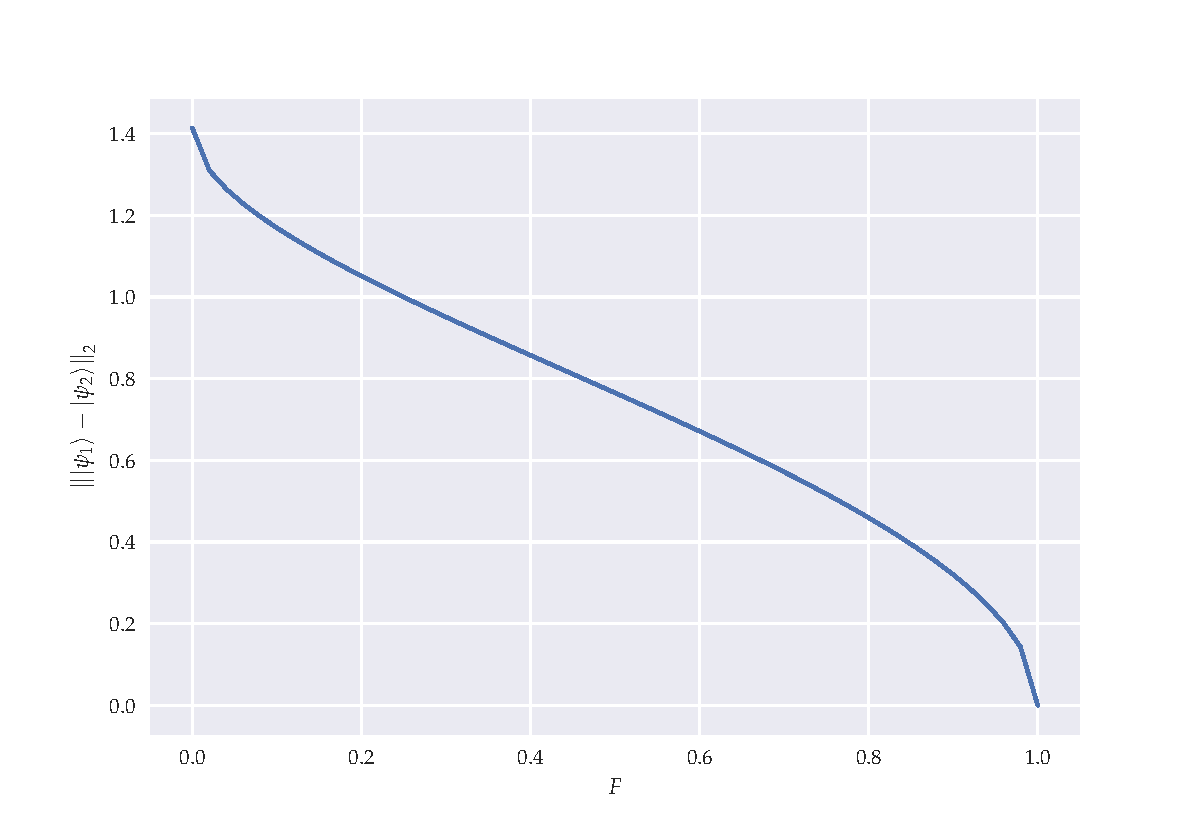
\includegraphics[width=0.7\textwidth]{figures/Fidelity.pdf}
    \caption{Norm of difference vs fidelity: a plot of equation \eqref{eq:norm-of-difference-fidelity}}
    \label{fig:fidelity}
\end{figure}

\section{Quantum teleportation}

It is possible to clone a generic quantum state \(\ket{\psi } = \alpha \ket{0} + \beta \ket{1}  \) assuming we start with two entangled qubits, one in the starting location and one at the destination: so, if these two qubits are called \(A\) and \(B\) and the state we want to transmit is in subsystem \(C\), we start with

\begin{equation}
    \qty(\frac{\ket{00} + \ket{11} }{\sqrt{2} })_{AB} \otimes \ket{\psi}_C
\end{equation}

The protocol is this:

\begin{enumerate}
    \item Apply the gate \(\text{C}_C\text{NOT}_A\); \label{step:cnot}
    \item apply the gate \(H_C\); \label{step:hadamard}
    \item measure \(A\) and \(C\) in the computational basis: call the result \(x\);
    \item apply a gate \(V_x\), selected according to table \ref{tab:teleportation-gate}, to \(B\).
\end{enumerate}

\begin{table}[H]
    \centering
    \begin{tabular}{c|c}
        \(x\) & \(V_x\) \\
        \hline
        00 & \(\mathbb 1\) \\
        01 & \(\sigma_z\) \\
        10 & \(\sigma_x\) \\
        11 & \(\sigma_z \sigma_x\)
    \end{tabular}
    \caption{Possibilities for gate \(V_x\). }
    \label{tab:teleportation-gate}
\end{table}

\begin{greenbox}
  Possibly, when Montangero wrote \(AC=01\) he meant \(A=1\) and \(C=0\).
\end{greenbox}

We can realize all of this with the gates \(\text{CNOT}\), Hadamard and \(\sigma_z\) (we can recover \(\sigma_x\) as \(\sigma_x = H \sigma_z H\).

\section{Quantum interferometry}

\paragraph{Beam splitter}

We call the sides of the BS \(A\) and \(B\), and denote the absence or presence of light on either side by \(\ket{0,1} _{A, B}\). Then the action of the beam splitter is unitary and can be represented in the partial basis \(\ket{0}_A \otimes \ket{1} _B , \ket{1}_A \otimes \ket{0} _B\) as

\begin{equation}
    U_{BS} = \frac{1}{\sqrt{2} }
    \begin{bmatrix}
    1   & i \\
    i   & 1
\end{bmatrix}
\end{equation}

Note that \(U_{BS}^2 = i\sigma_x\) in the BS-side basis: if we build a Mach-Zender interferometer, that is, we chain two beam-splitters, the light from the two paths interferes and we get some only on one side of the BS (the side opposite of the starting one).

\paragraph{Bomb detection}

If we block one of the paths between the detectors, around half of the time the light will hit this obstacle (our `bomb'). Around half the time it will go to the second BS, and then a quarter of the time it will be detected on either side of the BS. On the other hand, if there is no obstacle, we will see photons \emph{only} on a certain side of the final BS.

So around \(\frac[i]{1}{4} \) of the time we will have detected the bomb without the photon actually \emph{having been there}.

\section{Zeno effect} \label{sec:zeno}

We will work with \(\hbar=1\).
We look of the \emph{survival probability} with which we will retain our starting state: if our evolution operator is \(U = \exp(-iHt) \), this probability is \(\P = A^*A\), where \(A = \braket{\psi_0}{\psi (t)} \) and \(\ket{\psi (t)} = U \ket{\psi _0} \).

How does this probability look like for small \(t\)? We can expand, for a small \(\delta{t}\):

\begin{equation}
    U \sim \mathbb 1 -i H \delta{t} - H^2 \delta t^2
\end{equation}

then we will have

\begin{equation}
    A = \bra{\psi_0}  \qty(\mathbb 1 -i H \delta{t} - H^2 \delta t^2) \ket{\psi_0}
    = 1 -i \expval{H}_0 \delta{t} - \frac{1}{2}  \expval{H^2} _0 \delta t^2
\end{equation}

so we can calculate \(\P\):

\begin{equation} \label{eq:zeno-probability}
    \P = \abs{1 -i \expval{H}_0 \delta{t} - \frac{1}{2} \expval{H^2} _0 \delta t^2}^2
    = 1 - \delta t^2 \qty(\expval{H^2} _0 - \expval{H}_0^2)
\end{equation}

Equation \eqref{eq:zeno-probability} is accurate to the order \(\delta t^3\), since we only ignored a fourth order term. The term multiplying \(\delta t^2\) can be interpreted as the inverse of a characteristic time:

\begin{equation}
    \tau = \frac{1}{\sqrt{\expval{H^2} _0 - \expval{H}_0^2}} = \frac{1}{\Delta H _0}
\end{equation}

\paragraph{Repeated measurements}

If we measure some observable with \(\ket{\psi _0}\) as an eigenspace, a fraction \(\frac[i]{t^2}{\tau^2} \) of the time we will get something different from \(\ket{\psi _0} \).

So, if in a long time \(t\) we measured \(N\) times, the probability of the system having remained in the original state is at least \(\P (t) \geq \P^N(\frac[i]{t}{N} )\): we consider the case in which the system remained in the state for \emph{all} the measurements. The latter pertains to a small time so we can apply equation \eqref{eq:zeno-probability}:

\begin{equation}
    \P \geq \P^N\qty(\frac{t}{N}) = \qty(1- \frac{t^2}{N^2 \tau^2} )^N
\end{equation}

if we fix the inverse of the measurement rate \(\frac[i]{N}{t} = R\) this becomes \(\P \geq x^t = \exp(t \log x) \), with \(x = \qty(1 - \frac[i]{1}{R^2\tau^2})^R\), so \(\log x =  R \log(1- \frac[i]{1}{R^2 \tau^2} ) < 0\). So, we call \(-\log x = \gamma_{\text{eff}}>0 \): then

\begin{equation}
    \P \geq e^{-\gamma _{\text{eff}} t }
\end{equation}

Note that as \(R \rightarrow \infty\), \(\gamma _{\text{eff}} \sim R^{-1}\tau^{-2}\).

\paragraph{An example of nonunitary evolution}

We consider a Hamiltonian like \(H = \Omega \sigma_x \), which might be that of a spin-$1/2$ particle, polarized along \(z\), in a magnetic field along \(x\). Say our system starts at \(\ket{\psi _0}  = \ket{0} \). Then the evolution looks like

\begin{equation}
    \exp(-iHt) \ket{0} = \cos(\Omega t) \ket{0} -i \sin(\Omega t) \ket{1}
\end{equation}

We can calculate the quantities from section \ref{sec:zeno}: \(A = \cos(\Omega t) \) and \(\P = \cos^2(\Omega t)\), for small \(t\):  \(\P \sim 1- \Omega^2  t^2\). We recognise the expression for the Zeno time: in this case \(\tau = \Omega^{-1}\)

Let us introduce the nonunitary part: we change \(H\) to

\begin{equation} \label{eq:interaction-hamiltonian}
    H _{\text{int}}  = \begin{bmatrix}
    -iV \\
    \Omega  \\
    0    \\
    +iV
\end{bmatrix}
    \cdot
    \begin{bmatrix}
    \mathbb 1 \\
    \sigma_x  \\
    \sigma_y  \\
    \sigma_z
\end{bmatrix}
    =
    -iV \mathbb 1 + \vec{h} \cdot \vec{\sigma}
    =
    \begin{bmatrix}
    0   & \Omega   \\
    \Omega  & -2iV
\end{bmatrix}
\end{equation}

to represent interaction with a second lower-energy system, to which our first one can decay \emph{if it is in the state \(\ket{1}\)}. Can we get a Zeno-like effect with this kind of interaction, and without \emph{measuring} anything?
The evolution of this new Hamiltonian will look like

\begin{equation}
    \exp(-itH) = e^{-tV} \exp(-it \vec{h} \cdot \vec{\sigma} ) = e^{-tV} \qty(\cosh(h t)\mathbb 1 -i \frac{\vec{\sigma} \cdot \vec{h} }{h} \sinh(ht) )
\end{equation}

where \(h = \sqrt{ V^2 - \Omega^2} \in \R\), since we assume the coupling is strong (\(V \gg \Omega\)).

This comes from the fact that for a unit vector \(\vec{n} \): \((\vec{n} \cdot \vec{\sigma})^n = \mathbb 1  )\) if \(N\) is odd, \(\vec{n} \cdot \vec{\sigma} \) otherwise: thus we can show that

\begin{equation}
    \exp(i \theta (\hat{n} \cdot \sigma )) = \cos(\theta) \id + i (\hat{n} \cdot \sigma) \sin(\theta )
\end{equation}

So, we can compute \(A = \expval{U} _0\):

\begin{equation}
    A = \frac{1}{2} \qty(1 + \frac{V}{h})e^{-(V-h)t}+
    \frac{1}{2} \qty(1 - \frac{V}{h})e^{-(V+h)t}
\end{equation}

\(V\) is close to \(h\) but slightly larger, so both the exponentials' arguments are negative.

For large times we can discard the quickly-decaying second exponential, and be left with

\begin{equation}
    \P = \abs{\frac{1}{2} \qty(1 + \frac{V}{h})e^{-(V-h)t}}^2
    \sim \qty(1 + \frac{\Omega^2}{2 V^2}) \exp(-t \frac{\Omega^2}{V})
\end{equation}

So, weird normalizations for small times aside, \(\gamma _{\text{eff}} = \Omega^2 /V \), but \(\Omega = \tau^{-1}\), so \(V = R\), the `rate of observation': the stronger the coupling, the more the other system influences ours.

\section{Non-unitary evolution}

It happens when the particle can escape the system; for example in optical systems there can be a complex index of refraction. The Hamiltonian will look like

\begin{equation}
    H = H_0 - iV \mathbb 1
\end{equation}

where \(V \in \R^+\). The unitary evolution has an \(i\) multiplying the Hamiltonian, so we get a decreasing real exponential.

We will have \(A \sim 1 -V \delta t + O(\delta t^2)\), so \(\P  \sim 1 - 2V \delta t + O(\delta t^2)\): the first derivative is nonzero!

\paragraph{An example of a nonhermitian Hamiltonian}

We consider a system and its environment together:

\begin{equation}
    H = \underbrace{\Omega \sigma_x}_{\substack{\text{system}}}  + \underbrace{\int   \dd{\omega} \dyad{\omega}}_{\substack{\text{environment}}} + \underbrace{\sqrt{\frac{\Gamma}{2 \pi}} \int   \dd{\omega} g(\omega) \qty(\ketbra{-}{\omega} + \ketbra{\omega}{-}  )  }_{\substack{\text{interaction}}}
\end{equation}

Where \(\sigma_x\) is meant to be in the \(\ket{-}, \ket{+}  \) basis. Now, let us take a generic state \(\ket{\psi } = x(t) \ket{-} + y(t) \ket{+} + \int \dd{\omega} z(\omega, t) \ket{\omega} \).

We will write the Schrödinger equation for the evolution of \(x\), \(y\) and \(z\) and show that, if we just consider the first two, the effective Hamiltonian looks like the one in \eqref{eq:interaction-hamiltonian}.

The system so solve can be separated into

\begin{subequations}
\begin{align}
  i \dot{x} &= \Omega y \\
  i \dot{y} &= \Omega x +\sqrt{\frac{\Gamma}{2 \pi}} \int z \dd{\omega}   \\
  i \dot{z} &= \omega z +\sqrt{\frac{\Gamma}{2 \pi}} y
\end{align}
\end{subequations}

In can be readiliy verified that, with starting conditions \(x=1\), \(y=z=0\), we have

\begin{equation}
    z(\omega, t) = -i \sqrt{\frac{\Gamma}{2 \pi}} \int _{0}   ^{t} \dd{\tau} y(\tau) e^{-i \omega (t-\tau)}
\end{equation}

so we substitute into the equation for \(y\)

\begin{equation}
    i \dot{y} = \Omega x  -i\frac{\Gamma}{2 \pi} \int \dd{\omega} \int _{0}   ^{t} \dd{\tau} y(\tau) e^{-i \omega (t-\tau)}
\end{equation}

but \(\int   \dd{\omega} e^{-i \omega (t- \tau)} = 2 \pi \delta(t- \tau)\): so

\begin{equation}
    i \dot{y} = \Omega x  -i\Gamma y(t) /2
\end{equation}

The factor \(1/2\) comes from the fact we integrated a \(\delta\) on the \emph{boundary} of the domain.
We can combine the results into

\begin{equation}
    i \dv{}{t} \begin{bmatrix}
    x \\
    y
\end{bmatrix}
    = \begin{bmatrix}
    0   & \Omega     \\
     \Omega  & -i \Gamma /2
 \end{bmatrix}
    \begin{bmatrix}
    x \\
    y
\end{bmatrix}
\end{equation}

\section{Implementation of quantum gates}

We want to implement a NOT gate (\(\sigma_x\)): we use a spin-$1/2$ particle, and two magnetic fields described by  a Hamiltonian

\begin{equation}
    H = - \mu \qty(B_0 \sigma_z + B_1 \qty(\cos(\omega t) \sigma_x + \sin(\omega t)\sigma_y  ))
\end{equation}

So the zeroth field is fixed on \(z\), while the other rotates around the \(z\) axis staying on the \(xy\) plane.

\begin{greenbox}
  TODO
\end{greenbox}

\section{Density matrices}

Say we have a generic observable \(\hat{A} = \sum _{i}  a_i \dyad{a_i} \), and our has a probability \(p_i\) of being in the state \(\ket{\psi_i}\): of course we must have \(\sum _{i}  p_i = 1 \). Then, we want to compute the expectation value \(\expval{A} \) in this ``mixed'' state: it will look like

\begin{subequations}
\begin{align}
   \expval{A} &= \sum _{i,k} p_i a_k \braket{\psi_i}{a_k}\braket{a_k}{\psi_i}   \\
   &= \sum _{i,j,k}  p_i a_k  \bra{a_k}\qty(\ketbra{a_j}{a_j})\ket{\psi_i} \braket{\psi_i}{a_k}  \\
   &= \sum _{k} \bra{a_k} \qty(\sum_j \underbrace{a_k}_{\substack{k\equiv j\text{ since it is }\\ \text{multiplied by }\delta_{jk}}}  \dyad{a_j} ) \qty(\sum_i p_i \dyad{\psi_i} ) \ket{a_k} \\
   &= \Tr \qty(A \rho) = \Tr \qty(\rho A)
\end{align}
\end{subequations}

So, we have defined

\begin{equation}
    \rho \defeq \sum _{k} p_k  \dyad{\psi_k}
\end{equation}

\paragraph{Properties}

\begin{enumerate}
    \item \(\Tr \rho = 1\)
    \item \(\rho = \rho^\dag\)
    \item \(\rho \geq 0\)
    \item \(\Tr \rho^2 \leq 1\)
\end{enumerate}

These can be deduced from writing the matrix elements \(\rho _{ij} = \bra{i} \rho \bra{j} \) in an ON basis, or by noticing that \(\rho \) is a positively-weighted sum of projectors, each of which is self-adjoint.

The first one needs the components approach, I think: \(\rho_{ii} = \sum _{ik}  \abs{\braket{\psi_k}{i} }^2 =1 \) since they are the components in a basis of a normalized ket.

The last property can be seen by noticing that \(\rho\) is self-adjoint, so it has an orthonormal basis: then squaring it is easy, and all the coefficients are such that \(p_i^2 \leq p_i\).

\paragraph{Time evolution of a density matrix}

How does \(\rho\) evolve? If we have \(U\), we can write the evolution by linearity as

\begin{equation}
    \rho(t) = \sum _{k} p_k  U\dyad{\psi_k}U^\dag =  U \rho_0 U^\dag
\end{equation}

If instead we wish to look at the differential formulation, starting from \(i \hbar \ket{\dot{\psi}_k} = H \ket{\psi_k}\) and its adjunct \(-i \hbar \bra{\dot{\psi}_k} =  \bra{\psi_k} H\) we get

\begin{equation}
    \dv{}{t} \rho(t) =  \sum _{k} p_k  \dv{}{t} \qty(\dyad{\psi_k})
    = \frac{1}{i \hbar} \sum _{k} p_k  \qty(H \dyad{\psi_k} - \dyad{\psi_k}H)
    = \frac{[H, \rho]}{i \hbar}
\end{equation}

\paragraph{Pure states}

A density matrix is a \emph{pure state} if it has only one component, in the sense that: \(\rho = \dyad{\psi} \). The following are equivalent:

\begin{enumerate}
    \item \(\rho \) is a density matrix;
    \item \(\rho\) has rank 1;
    \item \(\Tr \rho^2 = 1\).
\end{enumerate}

The quantity \(\Tr \rho^2\) is called the \emph{purity}, and is surely greater than \(1/d\), \(d\) being the dimension of the Hilbert space (consider \(\rho = d^{-1} \mathbb 1\)).

\paragraph{Examples of density matrices}

For a single pure qubit:

\begin{equation}
    \rho = \dyad{\psi} = \begin{bmatrix}
    \cos^2(\theta/2)    & \cos(\theta/2) \sin(\theta/2) e^{-i \varphi}    \\
     \cos(\theta/2) \sin(\theta/2) e^{i \varphi}  & \sin^2(\theta/2)
 \end{bmatrix}
\end{equation}

For a generic one-qubit mixed state:

\begin{equation} \label{eq:bloch-representation-density-matrix}
    \rho =
    \frac{1}{2} \qty(\id + \vec{r} \cdot \vec{\sigma}  )
    =\frac{1}{2}\begin{bmatrix}
    1 \\
    x  \\
    y    \\
    z
\end{bmatrix}
    \cdot
    \begin{bmatrix}
    \mathbb 1 \\
    \sigma_x  \\
    \sigma_y  \\
    \sigma_z
\end{bmatrix}
    = \frac{1}{2} \begin{bmatrix}
     1+z  & x-iy \\
     x+iy  & 1-z
 \end{bmatrix}
\end{equation}

it can be shown by direct computation that in this case \(\Tr \rho^2 = \frac[i]{1}{2} (1+\abs{r}^2) \),where \(\vec{r} = (x, y, z) \): so the state is pure for \(\abs{\vec{r}}=1 \), and the purity is quadratic in \(\abs{\vec{r}}\).

We could also look at \(\det \rho = \frac[i]{1}{4} (1-\abs{r}^2)\) and see that it is zero when \(\abs{\vec{r} }=1 \), but that method seems less powerful...

\paragraph{Composite systems}

Say we have two Hilbert spaces 1 and 2, with their respective orthonormal bases \(\ket{i} \) and \(\ket{\alpha} \) respectively (let us work with finite-dimensional ones for simplicity).

Say we want to calculate the expectation value of an observable \(A_1\) on 1: we must write it as \(A_T = A \otimes \id_2\).
Of course, our density matrix will also have four indices.
Then

\begin{equation}
    \expval{A} = \Tr \qty(\rho A_T)
    = \sum _{k \gamma} \bra{k \gamma}
    \qty(\sum _{ij \alpha \beta} \rho_{i \alpha}^{j \beta}  \ketbra{i \alpha}{j \beta})
    %\qty( A \otimes \id_2)
    \qty(\sum_{mn \sigma \xi} A_m^n \delta_ \sigma^ \xi \ketbra{m \sigma}{n \xi})
    \ket{k \gamma}
\end{equation}

So we can make the sums implicit,  the components of \(A\) explicit, and simplify some \(\delta\)s:

\begin{equation}
    \Tr \qty(\rho A_T)
    = \delta_k^i \delta_\gamma ^\alpha
    \rho_{i \alpha}^{j \beta}
    \delta_j ^m \delta_\beta^\sigma
    A_m^n \delta_ \sigma^ \xi
    \delta_n^k \delta_\xi^\gamma
    %= \rho_{i \alpha}^{j \beta} A_m^i \delta_{\beta}^\alpha  \delta^m_k   \delta_j^k
    = \rho_{i \alpha}^{j \alpha} A_j^i
\end{equation}

The simplifications are easier to understand by writing the index equivalencies:
\(m \equiv j\), \(i \equiv k \equiv n\) and \(\alpha \equiv \gamma \equiv \xi \equiv \sigma \equiv \beta\).

The trace with a simple one-subsystem density matrix, with the same one-subsystem observable \(A\), would look like

\begin{equation}
    \Tr \qty(\rho A) = \rho_i ^j A_j^k \delta_k ^i = \rho_i^j A_j^i
\end{equation}

So it becomes clear that we can use the traced matrix \(\rho_{i \alpha}^{j \alpha} \defeq (\rho_1)_i^j\) as a \emph{reduced density matrix} for the first subsystem.

We can write this in index-free notation as

\begin{equation} \label{eq:reduced-density-matrix}
    \rho_1 = \Tr_2 \rho
\end{equation}

Note that even when \(\rho\) is a pure state, if we trace out a subsystem it can become mixed: this can be seen with \(\rho = \frac[i]{1}{2} (\ket{00} + \ket{11})(\bra{00} + \bra{11})\), whose \(\rho_1 = \frac[i]{1}{2} (\dyad{0} + \dyad{1})\).

\section{Correlations}

We want to characterize quantum observables \(x\) and \(y\). Let us start by defining the standard deviation:

\begin{equation}
    \sigma_x = \sqrt{\expval{\qty(x - \expval{x} )^2}}
\end{equation}

So, we can define the covariance between two variables:

\begin{equation}
    C_{xy} = \frac{\expval{(x - \expval{x}) (y - \expval{y} )}}{\sigma_x \sigma_y}
    = \frac{\expval{xy} - \expval{x} \expval{y} }{\sigma_x \sigma_y}
\end{equation}

(Unless \([x,y]=0\) this is not the same as \(C_{yx}\)!)

\section{Schmidt decomposition}

Let us take a generic state in a two-subsystem system: \(\ket\psi = \sum _{i, \alpha} c_{i \alpha} \ket{i}_A \ket{ \alpha}_B \). In general, this will be a superposition of \(\dim A \dim B\) states. Schimdt  says we can write it as

\begin{equation}
    \ket{\psi}
    = \sum _{i=1} ^k \sqrt{p_i}  \ket{i}_A \ket{\alpha(i)} _B
\end{equation}

where \(k\) is called the \emph{Schmidt rank}, and the \(\ket{\alpha(i)} \) are orthormal. Also, \(p_i \geq 0\) and \(\sum _{i} p_i = 1 \).

How do we get this? We start from our generic state and rewrite it:

\begin{subequations}
\begin{align}
  \ket\psi &=  \sum _{i, \alpha} c_{i \alpha} \ket{i}_A \ket{ \alpha}_B  \\
  &= \sum _{i}  \ket{i} \qty(\sum _{\alpha} c_{i \alpha} \ket{\alpha})  \\
  &= \sum _{i}  \ket{i} \ket{\widetilde{\alpha} (i) } \label{eq:two-subsystem-schmidt-state-nonnormalized}
\end{align}
\end{subequations}

This seems fine,  but the \(\ket{\widetilde{\alpha}(i) } \) do not have the properties we want: they are not orthonormal.
Let us use equation \eqref{eq:reduced-density-matrix}, with an explicit one-subsystem matrix, and set it equal to the density matrix of \eqref{eq:two-subsystem-schmidt-state-nonnormalized}.

\begin{subequations}
\begin{align}
  \sum _{i} p_i \dyad{i}   &= \Tr_2 \qty(\sum _{i,j}  \ket{i} \ket{\widetilde{\alpha} (i)} \bra{j} \bra{\widetilde{\alpha }(j)})  \\
  &= \sum _{\gamma} \bra{\gamma}  \qty(\sum _{i,j}  \ket{i} \ket{\widetilde{\alpha} (i)} \bra{j} \bra{\widetilde{\alpha }(j)}) \ket{\gamma}  \\
  &= \sum _{i,j}  \ket{i}\bra{j}
  \qty(\bra{\widetilde{\alpha} (i)} \qty(\sum _\gamma \dyad{\gamma})  \ket{\widetilde{\alpha }(j)})^*  \\
  &= \sum _{i,j}  \ket{i}\bra{j}
  \braket{\widetilde{\alpha} (j)}{\widetilde{\alpha} (i)}
\end{align}
\end{subequations}

So, in order for the equality to work it must be that \(\braket{\widetilde{\alpha} (j)}{\widetilde{\alpha} (i)} = p_i \delta_{ij}\). So, we can rewrite equation \eqref{eq:two-subsystem-schmidt-state-nonnormalized} with \(\ket{\widetilde{\alpha}(i) }  \rightarrow  \ket{\widetilde{\alpha} (i) } / \sqrt{p_i} \), which are orthonormal.
So, we get

\begin{equation}
    \ket{\psi} = \sum _{i} \sqrt{p_i}  \ket{i} \ket{\widetilde{\alpha} (i) }
\end{equation}

and the properties of the \(p_i\) are inherited from the one-subsystem matrix.

Note that the Schmidt rank is very susceptible to small perturbations.

\paragraph{Correletions for separable states}

A separable state can be written as \(\ket{\psi} = \ket{i}_A \ket{\alpha}_B\). If we have an observable on either system, then the correlation will be zero, since the averaging in \(\expval{x_Ay_B} \) will factor.

\paragraph{Purification} \label{par:purification}

If we have a generic state \(\rho = \sum _{i} p_i \dyad{i}  \), we can add a second subsystem in order to make it into a pure state: let us call the full density matrix \(\sigma = \dyad{\psi} \), which must equal \(\rho\) if we trace out the second system. The components of \(\sigma\) will look like \(\sigma_{i \alpha} ^{j \beta} = c_{i \alpha} c^*_{j \beta}\), \(c\) being the components of \(\ket{\psi } \) in the two-system basis.

\begin{subequations}
\begin{align}
    \rho &= \sum _{\gamma}  \bra{\gamma}
    \qty(\sum _{ij \alpha \beta} \sigma_{i \alpha} ^{j \beta} \ket{i \alpha} \bra{j \beta}   )
    \ket{\gamma}  \\
    &= \sum _{ij \alpha \beta} \sigma_{i \alpha} ^{j \beta} \ket{i} \bra{j} \braket{\beta}{\alpha}  \\
    \sum _{ij} \rho_{ij} \ketbra{i}{j} &= \sum_{ij \alpha \beta} c_{i \alpha} c^*_{j \beta} \delta_ \alpha ^ \beta \ketbra{i}{j}
\end{align}
\end{subequations}

So the equation to be solved is \(\rho_{ij} = c_{i \alpha} c_{j \alpha}^*\): these are \((\dim A)^2\) equations, and we have \((\dim B)^2\) parameters to tweak: so this can always be done with \(\dim B = \dim A\).

\section{Kraus representation}

How does a subsystem \(\rho_1\) of \(\rho = \rho_1 \otimes \dyad{G}_2 \) evolve? We are using a pure state for subsystem 2 but the construction will be general, since as we saw in \Nameref{par:purification} we can purify states.
We know that \(\rho(t) = U \rho U^\dag\), so:

\begin{equation}
    \rho_1(t) = \Tr_{2} \qty(U\qty(\rho_1 \otimes \dyad{G}_2 )U^\dag)
    = \sum _k \bra{k} U \ket{G} \rho_1 \bra{G} U^\dag \ket{k}
\end{equation}

so we define \(E_k = \bra{k} U \ket{G}\). Note that this is still a matrix, since we only contracted the subsystem 2 indices. These matrices obey \(\sum _{k}  E_k ^\dag E_k = \id\).
With this, we get

\begin{equation}
    \rho_1 (t) = \sum _{k} E_k \rho_1 E_k ^\dag
\end{equation}

This defines a \emph{superoperator} \(\mathcal S: \rho \rightarrow \sum _k E_k \rho E_k ^\dag \).

Because of how it was defined, \(\mathcal S\) has the following properties:

\begin{enumerate}
    \item it preserves self-adjointness; \label{item:superoperator-prop-1}
    \item it preserves the trace;\label{item:superoperator-prop-2}
    \item it preserves non-negativity.\label{item:superoperator-prop-3}
\end{enumerate}

The set of the \(\mathcal S\) also has a group structure, and \(\mathcal S^{-1}\) exists iff \(\mathcal S\) is unitary.

\paragraph{Kraus representations}

Any superoperator with properties \ref{item:superoperator-prop-1}, \ref{item:superoperator-prop-2} and \ref{item:superoperator-prop-3} it  can be written as

\begin{equation} \label{eq:kraus-superoperator}
    \mathcal S (\rho) = \sum _k E_k \rho E_k ^\dag
\end{equation}

\section{Generalized measurements}

A generalized measurement is defined by a set of operators \(M_i\), such that \(\sum _i M_i ^\dag M_i = \id\). They represent the possible results of the measurement: the wavefunction is reduced to

\begin{equation}
    \frac{M_i \ket{\psi}}{\norm{M_i \psi}}
    \qquad
    \text{with probability}
    \qquad
    p_i=
    \norm{M_i \ket{\psi}}^2
    = \bra{\psi} M_i ^\dag M_i \ket{\psi}
\end{equation}

Note that the probabilities are normalized: \(\sum _i p_i = 1\).

If all the \(M_i\) are projectors (\(M_i = M_i ^\dag = M^2_i\)) then we get the usual Von Neumann projective measurements.

\paragraph{Naimark Theorem}

Generalized measurements are equivalent to projective measurements in a larger space: more specifically, a generalized measurement is equivalent to:

\begin{enumerate}
    \item Adding some ancillary qubits;
    \item evolving the whole system unitarily;
    \item taking a projective measurement.
\end{enumerate}

\subparagraph{Unitary characterization of Kraus evolution}

We have a Kraus evolution \(\rho \rightarrow \sum _{k}  E_k \rho E_k ^\dag \), with \(\sum _{k}  E_k ^\dag E_k = \id \).

Let us introduce a subsystem 2, with dimension the number of Kraus operators, and its orthonormal basis \(\ket{k} \), and the operator

\begin{equation}
    U \ket{\psi}_1 \ket{0}_2 \defeq \sum _{k}  E_k \ket{\psi}_1 \ket{k} _2
\end{equation}

\begin{claim}
\(U\) as defined is unitary.
\end{claim}

\begin{proof}
We can show this by proving \(\bra{\psi 0} U ^\dag U \ket{\psi 0} = 1  \).
This is then just a calculation:

\begin{equation}
    \bra{\psi 0} U ^\dag U \ket{\psi 0} =
    \sum _{k, k'} \bra{\psi}_1 \bra{k'}_2 E_{k'}
    E_k \ket{\psi}_1 \ket{k} _2
    = \bra{\psi}_1 \qty(\sum _{k}  E_k ^\dag E_k ) \ket{\psi}_2
    = 1
\end{equation}
\end{proof}

\begin{claim}
Taking the Kraus evolution of \(\rho_1 = \dyad{\psi}\) is equivalent to evolving \( \rho = \dyad{\psi 0} \) according to \(U\) and then tracing out subsystem 2.
\end{claim}

\begin{proof}
The evolution of \(\rho\) is \( \sum _{k, m}  E_k \ket{\psi}_1 \ket{k} _2
 \bra{\psi}_1 \bra{m} _2 E_m ^\dag\). Let us take the trace of this wrt subsystem 2: we get

\begin{equation}
     %\Tr_2 \sum _{k, m}  E_k \ket{\psi}_1 \ket{k} _2
     %\bra{\psi}_1 \bra{m} _2 E_m ^\dag =
     \sum _{j} \bra{j}_2  \qty(\sum _{k, m}  E_k \ket{\psi}_1 \ket{k} _2
      \bra{\psi}_1 \bra{m} _2 E_m ^\dag) \ket{j}_2
      = \sum _{k} E_k \dyad{\psi}_1 E_k ^\dag
      = \sum _{k} E_k \rho_1 E_k ^\dag
\end{equation}
\end{proof}

\begin{claim}
Evolving \(\ket{\psi} \ket{0} \) according to \(U\) and then taking a projective measurement is equivalent to a generalized measurement on subsystem 1.
\end{claim}

\begin{proof}
We take the measurement \(P = \id_1 \otimes \dyad{i} _2\).

\begin{subequations}
\begin{align}
  \Tr_{12} (\rho P_i) &= \sum _{jq} \bra{j} _1 \bra{q} _2
  \qty(\sum _{k, m}  E_k \ket{\psi}_1 \ket{k} _2
  \bra{\psi}_1 \bra{m} _2 E_m ^\dag)
  \qty(\id_1 \otimes \dyad{i}_2 )
  \ket{j} _1 \ket{q} _2  \\
  &= \sum _{j} \bra{j} _1
  \qty( E_i \dyad{\psi}_1  E_i ^\dag  )
  \ket{j} _1  \\
  &= \Tr_1 \qty(\dyad{\psi} E_i ^\dag E_i )
\end{align}
\end{subequations}
\end{proof}

\paragraph{Weak measurements}

We wish to measure a system without disturbing it too much: let us consider a System-Environment couple of qubits, in the initial state \(\ket\psi = \qty(\alpha \ket{0} + \beta \ket{1} )_S \otimes \ket{0} _E = \alpha \ket{00} + \beta \ket{10} \). We apply the gate

\begin{equation}
    U = (R_z (\theta)_S \otimes \id_E ) \qty(\cos(\theta) \id_{SE} - i \sin(\theta)
    \text{C}_S\text{NOT}_E  )
    = \begin{bmatrix}
    1   &   &   &  \\
       & 1  &   &  \\
       &   & e^{i \theta} \cos \theta   & - ie^{i \theta} \sin \theta   \\
       &   &  - ie^{i \theta} \sin \theta  & e^{i \theta} \cos \theta
   \end{bmatrix}
\end{equation}

\begin{greenbox}
    (Why is the phase included?)
\end{greenbox}

(\(\theta\) is small).
The result of the application of this gate to \(\ket{\psi} \) is

\begin{equation}
    U \ket{\psi}
    = \alpha \ket{00} + \beta e^{i \theta} \qty( \cos(\theta) \ket{10} -i \sin(\theta) \ket{11}  )
\end{equation}

Now, we measure the environment: we will most likely (with probability \(\sim 1- \abs{\beta}^2 \theta^2 \)) get \(0\): in this case the system is reduced to

\begin{equation}
    \frac{\alpha \ket{00} + \beta e^{i \theta} \cos(\theta) \ket{10}}
    {\sqrt{\abs{\alpha}^2 + \abs{\beta \cos(\theta) }^2  } }
\end{equation}

which approaches \(\ket\psi\) as \(\theta \rightarrow 0\).
If, instead, we get 1, the state becomes \(\ket{11}\).

This does not seem very useful, as it can only provide us with some statistical bounds on the size of \(\beta\) if we measure a few times, but we must not do it too often...

\subsection{POVMs} \label{subsec:POVM}

We get some set of positive operators \(F_i\) such that \(\sum _{i}  F_i = \id \), and use these as the possible results of our measurement, which we will get with probabilities \(p_i = \ev{F_i}{\psi}\), or more generally \(p_i = \Tr(\rho F_i)\).

They are useful in describing destructive measurements, like a photodetector.
It is interesting when \(p_i = 0\) with some \(\psi\), because if we see that detector go off we know the system was \emph{not} in \(\psi\).

\section{Quantum channels}

\paragraph{An example of decoherence by interaction}

If our first system starts in \(\ket{\psi} = \alpha \ket{0} + \beta \ket{1} \), so

\begin{equation}
    \rho = \begin{bmatrix}
    \abs{\alpha}^2   & \alpha  \beta ^*  \\
     \alpha ^* \beta   & \abs{\beta}^2
 \end{bmatrix}
\end{equation}

Now, let us consider a second subsystem, so the state becomes \(\alpha \ket{00} + \beta \ket{10}\), then we apply a CNOT gate controlling on our first subsystem: the state becomes \(\alpha \ket{00} + \beta \ket{11}\). If we trace the second subsystem out, the density matrix becomes

\begin{equation}
    \rho' = \begin{bmatrix}
    \abs{\alpha}^2   & 0  \\
     0   & \abs{\beta}^2
 \end{bmatrix}
\end{equation}

\paragraph{Linear transformations in Bloch space}

We take a Kraus transformation of a density matrix as given in equation \eqref{eq:kraus-superoperator}, and represent it as in equation \eqref{eq:bloch-representation-density-matrix}:  \(\rho = \frac[i]{1}{2} \qty(\id + \vec{r} \cdot \vec{\sigma} )\) (and in the same fashion \(\rho'\) with \(r'\)).

\begin{claim}
This Kraus transformation corresponds to a linear map \(r_i \rightarrow M_i^j r_j + c_i\) which is a contraction.
\end{claim}

\begin{bluebox}
\begin{proof}
We can expand the Kraus matrices as \(E_k = \gamma_k \id + \sum _{i} a_{ik} \sigma_i \): our full expression becomes

\begin{equation}
    \rho \rightarrow \rho' =
    \sum _{k}
    \qty(\gamma_k \id + \sum _{i} a_{ik} \sigma_i)
    \frac{1}{2} \qty(\id + \vec{r} \cdot \vec{\sigma})
    \qty(\gamma_k^* \id + \sum _{j} a_{jk}^* \sigma_j ^\dag)
\end{equation}

and our claim is that

\begin{equation}
    \rho' =
    \frac{1}{2} \qty(\id + \qty(M_i^j r_j + c_i) \sigma_i)
\end{equation}

for some matrix \(M_i^j\) and vector \(c_i\).
This can be readily seen by noticing that:

\begin{enumerate}
    \item products of Pauli matrices are linear combinations of Pauli matrices: \(\sigma_a \sigma_b = \delta_{ab} \id + i \varepsilon_{abc} \sigma_c\);
    \item the Kraus transformation sends density matrices into density matrices, so the trace of \(\rho'\) will still be \(1\) and we will be able to separate the trace term \(\id/2\) from the traceless Pauli matrix part (that is, there will not be any transformation-dependents coefficients multiplying the identity).
\end{enumerate}

Now, to see that it is a contraction recall that \(\Tr \rho^2 \leq 1\). We will apply the formula:

\begin{equation}
(\vec{a} \cdot \vec{\sigma}) (\vec{b} \cdot \vec{\sigma}) = (\vec{a} \cdot \vec{b}) \id  + i (\vec{a} \wedge \vec{b}) \cdot \vec{\sigma})
\end{equation}

So then:

\begin{equation}
    \Tr (\rho')^2 =
    \Tr \qty( \frac{1}{4} \qty(\id + \vec{r'} \cdot \vec{\sigma})^2)
    = \Tr\qty( \frac{1}{2} \qty(\frac{1 + \abs{r'}^2 }{2} \id + \vec{r'} \cdot \vec{\sigma}))
\end{equation}

therefore \(\abs{r'} \leq 1\): the image of the unit sphere is contained in the unit sphere.
\end{proof}
\end{bluebox}

We can write explicit equations for \(M\) and \(c\):

\begin{subequations}
\begin{align}
    M_{jk} &= \sum _{l} \qty(
    2 \Re \qty(a_{lj} a_{lk}^*)
    + \delta_{jk} \qty(
    \abs{\gamma_l}^2 - \sum _p \abs{a_{lp}}^2
    )
    + 2 \sum _p \varepsilon_{jkp} \Im \qty(
    \gamma_l ^* a_{lp}
    )
    )  \\
    c_j &= 2i \sum _{klm} \varepsilon_{jlm} a_{kl} a^* _{km}
\end{align}
\end{subequations}

It seems like it should be true that \(\abs{\det M} = 1 \) (and \(\vec{c} = 0\)) iff there is only one \(E_k\), that is, the channel is actually a unitary transformation.

\paragraph{*-flip channel}

\begin{equation}
    \mathcal S ( \rho) =
    \abs{\alpha}^2 \sigma_i \rho \sigma_i ^\dag + \qty(1 - \abs{\alpha}^2 ) \rho
\end{equation}

So \(E_0 = \alpha \sigma_i\) and \(E_1 = \sqrt{1 - \abs{\alpha}^2 } \id\).

\begin{enumerate}
    \item \(i=x\): bitflip
    \item \(i=z\): phaseflip
    \item \(i=y\): bitphaseflip
\end{enumerate}

In the Bloch sphere, it keeps the dimension \(i\) still and shrinks along the other two by a factor \(1- 2\abs{\alpha}^2 \). For example, the bitflip gate approaches \(\sigma_x\) as \(\abs{\alpha}^2  \rightarrow 1\).

This circuit can be represented as unitary evolution: we add a subsystem with a wavefunction \(\ket{\psi} = \alpha \ket{1} + \sqrt{1- \abs{\alpha}^2 } \ket{0} \), and perform a control-\(\sigma_i\) (where the new subsystem is the controller).

\begin{greenbox}
  In the expression of \(\psi\) the 0 and 1 are swapped, right?
\end{greenbox}

\paragraph{Depolarizing channel}

It mixes states: the fixed point is \(r = 0\).

\begin{equation}
    \mathcal S(\rho) = \frac{P}{3}\qty(\sum _i \sigma_i \rho \sigma_i ^\dag ) +
    \qty(1-P) \rho
\end{equation}

\begin{equation}
    r \rightarrow r \qty(1 - \frac{4P}{3})
\end{equation}

\paragraph{Amplitude damping channel}

Its Kraus matrices are

\begin{equation}
    E_0 = \begin{bmatrix}
    1   & 0 \\
    0   & \sqrt{1- P}
\end{bmatrix}
    \qquad
    E_1 = \begin{bmatrix}
    0   & \sqrt{P}  \\
     0  & 0
 \end{bmatrix}
\end{equation}

It moves the population towards \(\dyad{0} \):  it maps \(\dyad{1}  \rightarrow P \dyad{0} + (1-P) \dyad{1}  \).

The fixed point is a pure state, so this channel can increase the purity of a state; however,  it is fundamentally an incoherent process.

\begin{bluebox}
  In the Bloch sphere, the amplitude damping channel looks like:

  \begin{equation}
      r \rightarrow \begin{bmatrix}
      \sqrt{1-P}    &   &  \\
         &  \sqrt{1-P}  &  \\
         &   & 1-P
     \end{bmatrix}
      r + \begin{bmatrix}
      0 \\
      0  \\
      P
  \end{bmatrix}
  \end{equation}

  So, for example,  \(r = - \hat{z} \rightarrow (2P-1) \hat{z} \).
  This transformation has only \((0,0,1)^\top\) as its fixed point.
\end{bluebox}

\paragraph{Phase damping channel}

It models what we might see if our particle was in a variable magnetic field: the phase of the particle is rotated by varying similar continuously distributed angles. We can write the phase gate as \(R_z(\theta) = \diag{e^{-i \theta/2}, e^{i \theta/2}}\). We assume the phase angles are normally distributed with variance \(\lambda\):

\begin{equation}
    p (\theta) = \frac{\exp(\frac{-\theta^2}{2 \lambda}) }{\sqrt{\pi \lambda} }
\end{equation}

then the channel looks like

\begin{equation}
    \rho \rightarrow \int _{-\infty}   ^{+\infty} R_z(\theta) \rho R_z(-\theta) p(\theta)  \dd{\theta}
\end{equation}

Now let us take a generic density matrix:

\begin{equation}
    \rho = \begin{bmatrix}
    P   & \alpha \\
     \alpha^*  & 1-P
 \end{bmatrix}
\rightarrow
\int   \dd{\theta}p(\theta) \begin{bmatrix}
P   & \alpha e^{-i \theta} \\
 \alpha^* e^{i \theta}  & 1-P
\end{bmatrix}
\end{equation}

and by putting together \(p(\theta) e^{\pm i \theta}\) we can complete the square to get a Gaussian integral (which equals one since the pdf is already normalized) times \(e^{-\lambda}\). So

\begin{equation}
    \rho' = \begin{bmatrix}
    P   & \alpha e^{-\lambda} \\
     \alpha ^* e^{-\lambda}  & 1-P
 \end{bmatrix}
\end{equation}

\begin{bluebox}
  This can be also be interpreted as repeated application of the channel with the Kraus matrices

  \begin{equation}
      E_0 = \sqrt{1-P} \begin{bmatrix}
      1   & 0 \\
      0   & 1
  \end{bmatrix}
      \qquad
      E_2 = \sqrt{P} \begin{bmatrix}
      0   & 0  \\
      0   & 1
  \end{bmatrix}
      \qquad
      E_2 = \sqrt{P} \begin{bmatrix}
      1   & 0  \\
      0   & 0
  \end{bmatrix}
  \end{equation}

which send

\begin{equation}
    \rho \rightarrow \begin{bmatrix}
    \rho_{00}    & \rho_{01}(1-P) \\
     \rho_{10}(1-P)  & \rho_{11}
 \end{bmatrix}
\end{equation}

and if \(P = \lambda \delta t\) for small \(\delta t\) and the interactions are very fast then \(\rho'_{01} \rightarrow (1-\lambda \delta t)^{t/\delta t} \sim e^{-\lambda t}\).

\end{bluebox}

\paragraph{Entanglement damping channel}

Let us consider a nice entangled couple of qubits, with \(\ket{\psi} = \frac[i]{1}{\sqrt{2}} \qty(\ket{01} + \ket{10} )   \). How can we break it? We will use the Kraus operators \(E_{1,2} = \id \otimes \diag{1, \cos(\theta) }\) or \(\id \otimes \diag{1, \sin(\theta) }\).

Then, the density matrix becomes:

\begin{equation}
    \frac{1}{2}
    \begin{bmatrix}
       &   &   &  \\
       & 1  &  1 &  \\
       &  1 &  1 &  \\
       &   &   &
   \end{bmatrix}
    \rightarrow
    \frac{1}{2}
    \begin{bmatrix}
       &   &   &  \\
       & 1  & \cos(\theta)   &  \\
       &  \cos(\theta)  & 1  &  \\
       &   &   &
   \end{bmatrix}
\end{equation}

If we trace out one subsystem, we get \(\rho_i = \frac[i]{1}{2} \id\), before and after the transformation.

\section{Master equation}

We want to describe the time evolution of a system with Kraus matrices:

\begin{equation}
    \rho(t) = \mathcal S (t, t_0) \qty[\rho]
    = \sum _{k=0}  ^{N-1} E_k \rho E_k ^\dag
\end{equation}

with \(N \leq \qty(\dim \mathcal H)^2 \). It must have the following properties:

\begin{enumerate}
    \item \(\mathcal S (t, t)=\id\);
    \item It should become the conventional unitary evolution if \(N=1\);
    \item at any time, we must have \(\sum _k E_k ^\dag E_k  = \id\). \label{item:condition-identity-kraus-matrices}
\end{enumerate}

How will these matrices look? We would like to assume \(E_0 = \id +\frac[i]{H}{i \hbar} \dd{t} \), but this will not work: let us add a term \(K \dd{t}\), with a self-adjoint \(K\).

The other \(E_k\) will then be \(L_k \sqrt{\dd{t}} \) to first order.

Expanding condition \ref{item:condition-identity-kraus-matrices} to first order gives:

\begin{equation}
    \qty(
    \qty(\id + \qty(\frac{H}{i \hbar} + \frac{K}{\hbar})\dd{t})
    \qty(\id + \qty(-\frac{H}{i \hbar} + \frac{K}{\hbar})\dd{t})
    +
    \sum _{k}  L_k ^\dag L_k
    )\dd{t} \overset{!}{=} \id \dd{t}
\end{equation}

So, we must have \(K = -\frac[i]{\hbar}{2} \sum _{k}  L_k ^\dag L_k  \) (indeed self-adjoint).
How will our density matrix evolve after \(\dd{t}\) then? We will assume \(\mathcal S(t+\dd{t}, t) [\rho] = \rho + \dot{\rho} \dd{t} + O (\dd{t}^2)\).

\begin{equation}
    \dot{\rho} = \frac{[H, \rho]}{i \hbar} + \frac{\qty{K, \rho}}{\hbar} + \sum _k L_k \rho L_k ^\dag
\end{equation}

We can plug in our formula for \(K\)  and compact the sums into one, to get the

\paragraph{Gorini–Kossakowski–Sudarshan–Lindblad equation}

\begin{equation}
    \dot{\rho} = \frac{[H, \rho]}{i \hbar}  + \sum _k \qty( L_k \rho L_k ^\dag  - \frac{1}{2} \qty{L_k ^\dag L_k, \rho})
\end{equation}

This works if the system has no memory. If, instead, the evolution depends not only on the present state but on events further past, we must use the

\subparagraph{Markovian version}

The form we show here is the diagonal one. We have the restriction that the \(L_k\) must be traceless.

\begin{equation}
    \dot{\rho} = \frac{[H, \rho]}{i \hbar}  + \sum _{k} \gamma_k \qty( L_k \rho L_k ^\dag  - \frac{1}{2} \qty{L_k ^\dag L_k, \rho} )
\end{equation}

\section{One-key cryptography}

The simplest paradigm: we have a key \(k\), decryption and encryption algorithms \(D\) and \(E\): if \(P\) is the clear-text message and \(C \) is the encrypted one then \(E_k (P) = C\) and \(D_k (C) = P\).

Even a very simple algorithm is secure if the key is longer than the message, private and only used once: for example, if we have \(n\) letters in our alphabet, we can do \(E_k P_i = (P_i - k_i)\mod n\) and \(E_k C_i = (C_i + k_i)\mod n\).

We can distribute the keys with \emph{Quantum Key Distribution}: there are different algorythms to do it, a modern one we will not treat uses entanglement and is called E91 since Eckert invented it. We will look at Bennet \& Brassard.

\paragraph{Quantum Key Distribution: BB84}

Alice wants to send Bob a secure string of ones and zeroes.

She selects two bases, say \(B_z = \qty{\ket{0}, \ket{1}}\) and \(B_x = \qty{H \ket{0}, H \ket{1}  }\) (where we use the Hadamard gate, see \Nameref{par:hadamard}).

At random, she chooses a basis with which to send each qubit, and keeps a record of the bases she used.

Bob receives the qubits and also measures them in a basis chosen between \(B_z\) and \(B_x\), and keeps a record of the bases he used.

After the communication is finished, they exchange in clear text the list of the bases they used, and discard the bits where they used a different basis.

Now they have a secure shared list of bits: if Eve were to try to measure the qubits in the middle, around half the time she'd collapse the state into the wrong basis. So, Alice and Bob just need to check a portion of the bits they \emph{should} share, and if they don't match then something is wrong: either there is too much noise, or somebody's listening in. Either way, they discard the whole key and try again.

\paragraph{Correction methods}

\begin{enumerate}
    \item First of all, we check on a part of our message the error rate \(R\): if \(R/N\) is large (\(\sim 1/2\)) then we discard everything.
    \item Now that we know \(R\),  we can choose some length \(\ell\) such that \(R \ell /N\) is still small: then, we do a parity check on every \(\ell\) long block.
    \item If we somehow know that Eve knows \(k\) bits of our message, we can still generate a key she will not be able to know: if we split our message into \(n-k-s\) snippets for some \(s\), she will be able to gather only \(O(2^{-s})\) bits of information: after splitting the message, our \emph{new} message is something like the parity of each snippet.
\end{enumerate}

\paragraph{Attack methods}

Eve cannot intercept the qubits and resend them, that's the point. There are some things she could do,  though:

\begin{enumerate}
    \item \textbf{translucent attack}: Eve operates unitarily on the passing qubits, entangling them with some qubits she keeps, and which she measures only \emph{after} Alice and Bob have communicated which basis they used. \\
    Surely she cannot completely \emph{clone} the passing qubit, but she might do some sneaky low-interference stuff.
    \item \textbf{collective attacks} on several qubits at once.
\end{enumerate}

\section{Dense coding}

Bob and Alice prepare two qubits together, in  \(\ket{\psi} = \text{CNOT} (H \otimes \id) \ket{00}  = \frac[i]{1}{\sqrt{2} } \qty(\ket{00} + \ket{11} ) \). Now Alice takes a qubit with her, and Bob keeps the other.

Now they are far apart. Alice wants to send two classical bits \(xy\). She chooses based on her two bits an operator between \(U_i = \qty{\id, \sigma_x, \sigma_z, \sigma_y}\) and applies it to her qubit.

The state becomes one of these:

\begin{subequations}
\begin{align}
  U_0 \ket\psi &= \frac{1}{\sqrt{2} } \qty(\ket{00} + \ket{11} ) \\
  U_1 \ket\psi &= \frac{1}{\sqrt{2} } \qty(\ket{10} + \ket{01} ) \\
  U_2 \ket\psi &= \frac{1}{\sqrt{2} } \qty(\ket{00} - \ket{11} ) \\
  U_3 \ket\psi &= \frac{1}{\sqrt{2} } \qty(\ket{10} - \ket{01} )
\end{align}
\end{subequations}

Now she sends her qubit to Bob, who still has his.

Bob applies \(\qty(\text{CNOT} (H \otimes \id))^{-1} = (H \otimes \id) \text{CNOT}\) to the qubits.

\begin{equation} \label{eq:cnot-hadamard-inverse}
    \qty(\text{CNOT} (H \otimes \id))^{-1}=
\left[\begin{matrix}1 & 0 & 0 & 1\\0 & 1 & 1 & 0\\1 & 0 & 0 & -1\\0 & 1 & -1 & 0\end{matrix}\right]
\end{equation}

Now, as can be seen by summing the combinations of rows of the matrix in \eqref{eq:cnot-hadamard-inverse} corresponding to the states \(U_i \ket{\psi} \), Bob's qubits will be in the state \(\ket{xy} \).

In the end, the protocol can be written as:

\begin{equation}
    (H \otimes \id)
    \text{CNOT}
    (U_i \otimes \id)
    \text{CNOT}
    (H \otimes \id)
    \ket{00}
    = \ket{i}
\end{equation}

\begin{bluebox}
  If we tried to do this with a mixed state, the application of \(\id\) and \(\sigma_z\) would give the same result (\(\frac[i]{1}{2} \qty(\dyad{00} +\dyad{11} )\)) as would \(\sigma_x\) and \(\sigma_y\) (\(\frac[i]{1}{2} \qty(\dyad{01} +\dyad{10} )\)). So, since there would be only two distinguishable states, only 1 bit would be transmitted.
\end{bluebox}

\section{Bell Inequalities} \label{sec:bell-inequalities}

Alice and Bob have some (entangled) state on their hands, and are separated by a space-like interval. Alice makes a measurement \(x\) and gets outcome \(a\), Bob makes a measurement \(y\) and gets outcome \(b\).

They repeat this several times, always with the same starting state. This whole experiment is then characterized by the function \(\P (ab | xy)\). In general we will have correlations, so \(\P (ab | xy) \neq \P(a|x) \P (b|y)\). If our theory is local, however, these cannot be explained by the transmission of information from Alice to Bob. Can we describe them by some local unknown (\emph{hidden}) variable which determines the measurement \emph{a priori}?

\begin{claim}
The results of a Bell experiment which are predicted by quantum mechanics \emph{cannot} be described by a hidden variable \(\lambda\) distributed according to some function \(q(\lambda)\), with an expression in the form:

\begin{equation} \label{eq:local-hidden-parameter}
    \P(ab | xy) = \int q(\lambda) \P(a|x; \lambda) \P (b|y; \lambda)  \dd{\lambda}
\end{equation}
\end{claim}

\begin{proof}
We prove the statement by contradiction. How do we calculate a correlation under our hypothesis?
To simplify, we assume \(a, b \in \qty{+1,-1}\) and \(x, y \in \qty{0, 1}\).
I will use the (improper) notation \(\dd{q} = \dd{\lambda} q(\lambda)\)

\begin{equation}
    \expval{a b}_{xy} =
    \sum _{ab} a b \P(ab | xy)
    = \int \dd{q}
    \qty(\sum_aa\P(a|x; \lambda) )
    \qty(\sum_bb\P(b|y; \lambda) )
\end{equation}

Therefore, \(\expval{a b}_{xy} = \int   \dd{q} \expval{a}_{x, \lambda} \expval{b}_{y,\lambda}  \). Subscripts, here, mean conditioning.

\subparagraph{Hidden variable inequality (CHSH)}

Now, we consider the following quantity:

\begin{equation} \label{eq:CHSH-def}
    S = \expval{ab}_{00} +
     \expval{ab}_{01} +
     \expval{ab}_{10} -
     \expval{ab}_{11}
\end{equation}

The minus sign is arbitrarily placed, it just matters that there is just one negative and three positive terms. We can show  that \(S \leq 2\): surely

\begin{equation}
    S \leq \int  \dd{q} \qty[
    \abs{\expval{b}_{0, \lambda} + \expval{b}_{1, \lambda}} \sup \expval{a}_{0, \lambda} +
    \abs{\expval{b}_{0, \lambda} - \expval{b}_{1, \lambda}} \sup \expval{a}_{1, \lambda}
    ]
\end{equation}

and, since the outcomes are \(\pm 1\),  for any \(\lambda\): \(\expval{a}_{x, \lambda} \leq 1 \) and \(\expval{b}_{y, \lambda} \leq 1 \), so

\begin{equation}
    S \leq \int  \dd{q} \qty[
    \abs{\expval{b}_{0, \lambda} + \expval{b}_{1, \lambda}} +
    \abs{\expval{b}_{0, \lambda} - \expval{b}_{1, \lambda}}
    ]
\end{equation}

WLOG we can assume \(\expval{b}_{0, \lambda} \geq \expval{b}_{1, \lambda} \geq 0\). Therefore the integrand is bounded by \(\expval{b}_{0, \lambda} + \expval{b}_{1, \lambda} +
\expval{b}_{0, \lambda} - \expval{b}_{1, \lambda} = 2 \expval{b}_{0, \lambda} \leq 2\).

The probability density of \(\lambda\) must be normalized: \(\int  \dd{q} = 1  \). So, the integrand is an upper bound for the integral, and we get \(S \leq 2\).

(This can be generalized to \(\abs{S} \leq 2 \)).

\subparagraph{Quantum CHSH violation}

We use as our observables the spin in different directions: if we have a vector \(\vec{a}\), then \(\hat{O}_a = \vec{a} \cdot \vec\sigma\). As our state we take the antisymmetric spin singlet, \(\ket{\psi } = \frac[i]{1}{\sqrt{2} }  \qty( \ket{01}- \ket{10} )\). We want to show that the correlation expectation value \(\expval{O_a \otimes O_b}_\psi \) is equal to \(-a \cdot b\). We only need to compute the central four elements of the 4x4 matrix \(O_a \otimes O_b\), which correspond to the \(01\) and \(10\) basis elements.

\begin{equation} \label{eq:reduced-spin}
    \qty[O_a \otimes O_b] _{\text{reduced}} = \begin{bmatrix}
    -a_z b_z   & (a_x + i a_y)(b_x - i b_y) \\
      (a_x- i a_y)(b_x + i b_y) & - a_z b_z
    \end{bmatrix}
\end{equation}

We compute the expectation value of the matrix in \eqref{eq:reduced-spin}:

\begin{subequations}
\begin{align}
    \expval{O_a \otimes O_b}_\psi &= \frac{1}{2} \begin{bmatrix}
    1 & -1
    \end{bmatrix}
    \begin{bmatrix}
    -a_z b_z   & (a_x + i a_y)(b_x - i b_y) \\
      (a_x- i a_y)(b_x + i b_y) & - a_z b_z
    \end{bmatrix}
    \begin{bmatrix}
    1 \\
    -1
\end{bmatrix}  \\
&= \frac{1}{2}\qty( -a_z b_z   - (a_x + i a_y)(b_x - i b_y)
  -(a_x- i a_y)(b_x + i b_y) + (- a_z b_z))  \\
&= - \vec{a} \cdot \vec{b} \label{eq:CHSH-pauli-scalar-product}
\end{align}
\end{subequations}

Now: we pick as our measurement with possible outcomes \(0, 1\) two \emph{pairs} of directions, and we call the result 0 if the spin is measured along the first, 1 if it measured along the second.

\begin{enumerate}
    \item For \(\vec{a} \), we call the result \(0\) if the spin direction is \(\vec{a}_0=  \hat{x} \) and 1 if the spin direction is \(\vec{a}_1=\hat{y} \);
    \item for \(\vec{b} \), we call the result \(0\) if the spin direction is \(\vec{b}_0=-(\hat{x} +\hat{y} )/\sqrt{2} \) and \(1\) if the spin direction is \(\vec{b}_1= -(\hat{x}+\hat{y})/\sqrt{2} \)
\end{enumerate}

So, we can compute \(S\) using equation \eqref{eq:CHSH-pauli-scalar-product}:

\begin{equation}
    S = \expval{ab}_{00} +
     \expval{ab}_{01} +
     \expval{ab}_{10} -
     \expval{ab}_{11}
     = \frac{4}{\sqrt{2}} = 2 \sqrt{2} > 2
\end{equation}
\end{proof}

\section{Nonlocal correlations}

We want to define \emph{probability spaces}. We will use the notation of section \nameref{sec:bell-inequalities}. If \(a,b\) can have \(\Delta \in \N\) values, and there are \(m \in \N \) possible measurements (\(x, y\)) we can make. Then, our correlations are a point \(\P(ab | xy)\) in some subset \(\mathcal P\) of \(\R ^{m^2 \Delta^2}\), bounded by:

\begin{enumerate}
    \item \(\forall x, y, a, b: \P (ab|xy)\geq 0\);
    \item \(\forall x, y\):
    \begin{equation}
        \sum_{a=1}^{\Delta} \sum_{b=1}^{\Delta} \P(ab|xy) = 1
    \end{equation}
\end{enumerate}

Now, we define some subsets of this space.

\paragraph{No-Signaling}

The set is called NS.
We impose a condition which means: \emph{no matter what we do with a measurement, it will not affect the other}:
\(\forall x, x', y, y', a\)

\begin{equation}
    \sum_{b=1}^{\Delta} \P(ab|xy) = \sum_{b=1}^{\Delta} \P(ab|xy')
    \qquad \qquad
    \sum_{a=1}^{\Delta} \P(ab|xy) = \sum_{a=1}^{\Delta} \P(ab|x'y)
\end{equation}

this implies \(\P(a|x) = \P(a|xy) = \sum_b\P(ab|xy)\).

\begin{greenbox}
  In the \(\Delta=2\) case, \(a, b = \pm 1\) the No-Signaling conditions become

  \begin{equation}
      \P(ab|xy) = \frac{1 + a \expval{A_x} + b \expval{B_y} + ab \expval{A_x B_y}  }{4} \geq 0
  \end{equation}

  so if \(A\) and \(B\) have zero average, \(1 \pm \expval{A_x B_y} \geq 0 \).

  What?
\end{greenbox}

\paragraph{Local correlations}

The set is called \(L\).
It is the set of correlations that can be written as in equation \eqref{eq:local-hidden-parameter}.

\paragraph{Quantum correlations}

The set is called \(Q\).

If we have some operators \(M_{a|x}\) and \(M_{b|y}\) in their respective Hilbert spaces, such that for each conditioning they still form a POVM (see \Nameref{subsec:POVM}), then \(Q\) is the set of the probabilities which can be expressed as

\begin{equation}
    \P(ab | xy) = \Tr (\rho_{AB} M_{a|x} \otimes M_{b|y})
\end{equation}

This is in the context of nonprojective measurements, but as we saw in \Nameref{par:purification} states can be purified so that everything we do is unitary. In that context,

\begin{equation}
    \P (ab|xy) = \ev{A_x \otimes B_y}{\psi}
\end{equation}

with some self-adjoint families of operators \(A_x\) and \(B_y\).

It can be useful to have \(A_x B_y\), a product of commuting observables \([A_x, B_y]=0\) on the same space, instead of \(A_x \otimes B_y\); these descriptions are surely equivalent in the finite-dimensional case, maybe the latter is more general in the infinite-dimensional one.

\paragraph{Shapes and inclusions}

Every one of these sets is of the same dimension, and it can be shown that \(NS\), \(L\) are polytopes while \(Q\)'s boundary is curved. Also, \(L \subset Q \subset NS \subset \mathcal P\).

They are all bounded, convex, closed. The planes which separate them are in general called Bell Inequalities.

\subparagraph{The $\Delta=2, m=2$ case}

We can have different linearly independent \(S\)s, (\(S\) being the one defined in \eqref{eq:CHSH-def}). In 2D (a projection?) we have: \(L\) is a square (\(\abs{S_x} \leq 2\), \(\abs{S_y} \leq 2\)), \(Q\) is a circle (\(\abs{S}^2 \leq 8 \)), \(NS\) is a square (\(\abs{S'_{x, y}} \leq 4 \), with \(S'_{x, y} = H S_{x, y}\) ($H$ is the Hadamard gate)).

\section{Entropy}

A message is a sequence of characters from an alphabet. If the alphabet is \(\mathcal A = \qty{a_i}_i\) and each of the characters in the alphabet appears with probability \(p_i\), we can define \(\mathcal A\)'s \emph{entropy} as

\begin{equation}
    H = - \sum _{i} p_i \log(p_i)
\end{equation}

with the convention \(0 \log 0 = 0\)

\paragraph{Noiseless coding: Shannon's theorem}

Given a \(k\)-long message, asyntotycally as \(k \rightarrow \infty\) there exists an encoding with which we can express each character of the message with \(H\) bits on average, or the whole message with \(kH\) bits.

If we take any encoding, it can only do as good as Shannon encoding, and no better (at least not \emph{in general}).

\paragraph{Von Neumann entropy}

We can define the entropy of a mixed state \(\rho\) as

\begin{equation}
    S_V = -\Tr \qty(\rho \log\rho )
\end{equation}

\begin{enumerate}
    \item For pure states we have \(S_V (\dyad{\psi} ) = 0\);
    \item \(S_V\) is invariant wrt unitary transformations;
    \item \(0 \leq S_V \leq \dim \mathcal H\).\footnote{Since \(\prod_{i=1}^{N} p_i^{-p_i} \leq N\).}
\end{enumerate}

\paragraph{Quantum Noiseless coding: Schumacher's theorem}

If our alphabet is now made of pure states, the probability distribution of a message will be some hyper-density matrix, \(\rho^{\otimes N}\).

Schumacher says: in the limit of infinite message length, we can always compress it with \(S_V\) bits per letter.

\section{Entanglement measurements}

We want a measurement \(E(\rho)\) which satisfies:

\begin{enumerate}
    \item If \(\rho\) is separable, then \(E(\rho)=0\);
    \item \(E(\rho) = E(U \rho U ^\dag)\);
    \item If we have
    a set of operators \(A_i \otimes B_i\), to each of which
    we associate a probability\linebreak[4]
     \(p_i = \Tr \qty((A_i \otimes B_i) \rho (A_i \otimes B_i)^\dag)\), and which can project the state into the normalized application of the Kraus operators \(\sigma_i = (A_i \otimes B_i) \rho (A_i \otimes B_i) ^\dag / p_i\), then
    \begin{equation}
        E(\rho) \geq \sum _{i}  p_i E(\sigma_i)
    \end{equation}
    \begin{greenbox}
    This means: the entanglement is invariant under local Kraus evolution: the systems cannot become \emph{more} entangled when evolving on their own.

    NOT CLEAR HOW
    \end{greenbox}
    \item If \(\rho = \rho_{A}\) is a pure state then \(E(\rho) = S_V(\rho_A)\).
\end{enumerate}

\paragraph{Entanglement of formation}

We can define

\begin{equation}
    E_F (\rho) = \min \sum_i p_i S_V(\rho_A^i)
\end{equation}

where the minimum is to be taken over all the possible decompositions \(\rho = \sum _{i}  p_i \dyad{\psi_i}\) and \(\rho_A^i = \Tr _B (\dyad{\psi_j}) \): so, we pick a decomposition, we trace out the second system and take the entropy.

\paragraph{Concurrence}

This only applies to two-qubit systems.

\begin{equation}
    C(\rho) = \max(0, \lambda_1 - \lambda_2 - \lambda_3 - \lambda_4)
\end{equation}

Where the \(\lambda_i\) are eigenvalues of \( \qty(\rho \sigma_y ^{\otimes 2})^2 \), taken in decreasing order.

\section{Quantum algorithms}

\subsection{Oracle interrogation}

We have an oracle function \(f(x): \qty{0,1}^n \rightarrow \qty{0,1}\) which is either \emph{constant} (always gives the same result) or \emph{balanced} (gives 0 for half of its inputs, and 1 for the other half).

With a classical computer, we'd need \(\max(\lfloor n/2 \rfloor,2)\) calls to the oracle in the worst case to be sure that it is one and not the other. With a quantum computer, we can do it in just one call.

Take \(n=1\) for simplicity.

Our unitary representation of an oracle must be invertible, so we take the input along:

\begin{equation}
    U_f \ket{x} \ket{y} \rightarrow \ket{x} \ket{f(x) \oplus y}
\end{equation}

where \(\oplus\) is the XOR binary gate. \(y\) is generic, it could be set to zero but we want a general gate. The algorithm is

\begin{enumerate}
    \item Start with \(\ket{xy} = \ket{01}\);
    \item apply \(H \otimes H\);
    \item apply \(U_f\);
    \item apply \(H \otimes \id\);
    \item measure the first qubit.
\end{enumerate}

First of all: \((H \otimes H) \ket{01} = (\ket{0} + \ket{1})(\ket{0} - \ket{1} )/2\). Now:

\begin{equation}
    U_f \ket{x} \otimes\qty(\frac{\ket{0} - \ket{1}}{\sqrt{2} }) = (-)^{f(x)} \ket{x} \otimes
    \qty(\frac{\ket{0} - \ket{1}}{\sqrt{2}})
\end{equation}

So after the application of the oracle gate, the first qubit's state has become

\begin{equation}
    \frac{1}{\sqrt{2}}\qty((-)^{f(0)} \ket{0} + (-)^{f(1)} \ket{1})
\end{equation}

and if we apply a Hadamard to it, it becomes

\begin{equation}
    \frac{1}{2} \qty(
    \qty((-)^{f(0)} + (-)^{f(1)}) \ket{0}
    \qty((-)^{f(0)} - (-)^{f(1)}) \ket{1}
    )
\end{equation}

therefore the state is \emph{surely} \(\ket{\psi}= [f(0)=f(1)] \ket{0} + [f(0) \neq f(1)]\ket{1} \).

\paragraph{$n$-qubit case}

We do the same thing as before, only with \(n\) qubits: \(\ket{x} = \ket{0}^{\otimes n}  \) at the start, so after the Hadamards we get

\begin{equation}
    H ^{\otimes (n+1)} \ket{x} \ket{y} = \frac{1}{2^{(n+1)/2}} \sum _{x=0}   ^{2^n-1} \ket{x}_1 \qty(\ket{0}- \ket{1})_2
\end{equation}

so after applying the oracle and another Hadamard we get

\begin{equation}
    H \qty(\frac{1}{2^{n/2}} \sum _{x=0}   ^{2^n-1} (-)^{f(x)} \ket{x})
\end{equation}

on the first qubit. Now, either \(f(x)\) is constant or it is balanced: if it is constant then this is just \(\ket{0} \). If it is not, then it is orthogonal (since at least one of the bits must be different): so we can just check whether the system is in \(\ket{0} \).

\subsection{Grover}

The classical complexity for a search in an unstructured database is \(O(N)\), with Grover's algorithm we get \(O(N^{1/2})\).

The problem looks similar to the oracle: now our \(f(x) = [x=\overline{x}]\) and we seek \(\overline{x} \). We explain the procedure with \(n=2\):

\begin{enumerate}
    \item Start with \(\ket{xy} = \ket{\vec{0}1}\);
    \item apply \(H ^{\otimes (n+1)} \);
    \item apply \(U_f\); \label{item:grover-step-oracle}
    \item apply \(D \otimes \id\);
    \item measure the \(\ket{x} \) state.
\end{enumerate}

as before, after applying step \ref{item:grover-step-oracle} we get

\begin{equation} \label{eq:grover-oracle-state}
    \ket\psi_1
    = \frac{1}{2^{n/2}} \sum _{x=0}   ^{2^n-1}
    (-)^{f(x)}\ket{x}
    = \frac{1}{2^{n/2}}\qty( \sum _{x=0}   ^{2^n-1}
    \ket{x}) - 2 \ket{\overline{x} }
\end{equation}

Now, \(D\) is \(\frac[i]{1}{2} \) of the matrix with -1 on the diagonal, and 1 in every other entry. Its eigenvectors are exactly the possible \(\ket{x} \) after the oracle, so after the application of \(D\) we get exactly \(\ket{\overline{x} } \).

This \(D\) can be made with the usual gates as \(H^{\otimes 2} \sigma_x^{\otimes 2} (\id \otimes H) \text{CNOT} (\id \otimes H) \sigma_x^{\otimes 2} H^{\otimes 2}\). Below is the Python code to verify that it works.

We will also need the matrix \(D'\), which is such that \(D = H^{\otimes 2} D' H^{\otimes 2}\). It turns out that \(D' = \eta_{\mu \nu}\) for a Minkowski flat spacetime.

\begin{lstlisting}[language=Python]
    import numpy as np
    H = 1/np.sqrt(2)* np.array([[1,1], [1,-1]])
    H2 = np.kron(H, H)
    sigma_x = np.array([[0,1], [1,0]])
    sigma_x2 = np.kron(sigma_x, sigma_x)
    CNOT = np.array([[1,0,0,0],[0,1,0,0],[0,0,0,1],[0,0,1,0]])
    idH = np.kron(np.identity(2), H)
    print('D = ', H2 @ sigma_x2 @ idH @ CNOT @ idH @ sigma_x2 @ H2)
    print('Dprime = ', sigma_x2 @ idH @ CNOT @ idH @ sigma_x2)
\end{lstlisting}

\paragraph{Arbitrary \(n\)}

This method only works for \(n=2\). In general, we have a state proportional \(\sum _{x=0}^{2^n-1} \ket{x} \ket{y}\), an oracle such that \(U_f \ket{\overline{x} }\ket{y}  = -\ket{\overline{x} }\ket{y} \) while \(U_f \ket{x}\ket{y}= \ket{x} \ket{y}   \) for all the other \(x \neq \overline{x}\).

Now, we can write \(D' = \id - 2 \dyad{0}_1 \): so \(D = \id - 2 \dyad{S}_1 \), with \(S = H^{\otimes 2} \ket{0} = \sum _{x=0}^{2^n-1} \ket{x}\).

Our main gate will be \(G = D U_f\). What does it do? first, it flips the component of the state along \(\ket{\overline{x}} \); then it flips the component along \(\ket{S} \).

We know for sure that \(\ket{S} \) and \(\ket{\overline{x} } \) are not orthogonal: the angle between them will have \(\cos(\varphi) = 2^{-n/2}\), the coefficient of \(\ket{\overline{x} } \) in \(\ket{S} \). We are interested in \(\pi /2 - \varphi\), which we will call \(\delta \theta\).

It can be shown by a simple geometric argument that the application of \(G\) sends a state which has an angle \(\theta\) from  the hyperplane \(\ket{\overline{x} }^\perp \) into a state with an angle \(\theta + 2 \delta \theta\). So, we need \(K\) applications of \(G\) to get \(\theta \rightarrow \pi /2\), with \(K = (\pi/2)/(2 \delta \theta)\): since \(\sin\delta\theta = 2^{-n/2} \) and the rest are constants, \(K = O(\sqrt{2^n})=O(\sqrt{N})\), where \(N\) is the database size.

\subsection{Quantum Fourier Transform}

We have \(n\) qubits, and their states are \(\ket{x} \) with \(x\) ranging from 0 to \(N-1\), with \(N = 2^n\).

\paragraph{Classical FFT}

The definition of the  discrete Fourier transform of a vector \(x_i\), with \(i = 0, \dots, N-1 \), \((N = 2^n)\) is

\begin{equation}
    X_k = \sum _{j=0}   ^{N-1} x_j \exp(-\frac{2 \pi ijk}{N})
\end{equation}

To do this in \(O(N \log N)\) instead of \(O(N^2)\), we split the sum into the even and odd parts:

\begin{equation}
    X_k =
    \sum _{j=0}   ^{N/2-1} x_{2j} \exp(-\frac{2 \pi i(2j)k}{N}) +
    \exp(-\frac{2 \pi ik}{N})
    \sum _{j=0}   ^{N/2-1} x_{2j+1} \exp(-\frac{2 \pi i(2j)k}{N})
\end{equation}

Or in other words

\begin{equation}
    \text{FFT}(x)_k = \text{FFT} (\text{even}(x))_k
    + \exp(-\frac{2 \pi ik}{N}) \text{FFT} (\text{odd}(x))_k
\end{equation}

Then, we can apply the same split for the FFT of the even and odd parts, and so on.

This split will happen \(\log N = n\) times, after which there will just be one term in the sum.
We have to to this computation once for every possible value of the result vector, so in the end the complexity is \(O(N \log N)\).

\paragraph{Quantum version}

We define

\begin{equation}
    \text{QFT}(\ket{J}) = \frac{1}{\sqrt{N}} \sum _{k=0}   ^{N-1}
    \exp(\frac{2 \pi i J k}{N}) \ket{k}
\end{equation}

where as usual \(\ket{k} = \ket{k_0 k_1 \dots k_{n-1}} \). So, we can rewrite this as a sum over all the \(k_\alpha\):


\begin{subequations}
\begin{align}
    \text{QFT}(\ket{J}) &= \frac{1}{\sqrt{N}} \prod_{\alpha=0}^{n-1} \sum _{k_\alpha=0}   ^{1}
    \exp(-\frac{2 \pi i J}{N}) \exp(\sum _{\alpha=0}   ^{n-1} k_\alpha 2^{n-\alpha-1} )  \ket{k}  \\
    &=  \frac{1}{\sqrt{N}} \prod_{\alpha=0}^{n-1} \sum _{k_\alpha=0}   ^{1}
    \exp(-2 \pi i J) \exp(\sum _{\alpha=0}   ^{n-1} k_\alpha 2^{-\alpha-1} ) \ket{k} \\
    &=  \frac{1}{\sqrt{N}} \prod_{\alpha=0}^{n-1} \sum _{k_\alpha=0}   ^{1}
    \exp(-2 \pi i J k_\alpha 2^{-\alpha-1} ) \ket{k} \\
    &=  \frac{1}{\sqrt{N}} \prod_{\alpha=0}^{n-1}
    \qty(\sum _{k_\alpha=0}   ^{1}
    \exp(-2 \pi i J k_\alpha 2^{-\alpha-1} ) \ket{k_\alpha}) \\
    &=  \frac{1}{\sqrt{N}} \prod_{\alpha=0}^{n-1}
    \qty(    \ket{0}_\alpha + \exp(-2 \pi i J 2^{-\alpha-1} ) \ket{1}_\alpha)
\end{align}
\end{subequations}

but in the \(\exp(-2 \pi i J 2^\alpha) \) the terms in the binary expansion of \(J\) with a power higher than \(\alpha\) will just make the term rotate by \(2 \pi \), doing nothing.

So, to the Least Significant Bit \(\ket{J_{n-1}}\) we just apply a Hadamard. To the second LSB \(\ket{J_{n-2}} \) we apply a Hadamard, and then a control-\(R_z(2 \pi i / 2^2)\). In general

\begin{equation}
    \ket{J_\alpha} \rightarrow  \bigotimes_{k=2}^{n-\alpha} (C_{\ket{J_{n-k+1}}} - R_z)(2 \pi i / 2^{k}) \otimes H \ket{J_\alpha}
\end{equation}

\subsection{Shor's algorithm}

It is a method to factor a product of large numbers.

\paragraph{Motivation: two-key RSA cryptography}

Alice wants to communicate a message \(P\) to Bob.
Bob generates a public key \( K _{\text{Pu}} \) and a private key \( K _{\text{Pr}}  \), he sends the public key \( K _{\text{Pu}} \) to Alice, who encodes the message with an algorithm \(E\) which depends on the public key:

\begin{equation}
  C = E _{K _{\text{Pu}} } (P) = P ^e \mod N
\end{equation}

where \( N \) is chosen such that \( N = pq \), with \( p, q \in \Z_{\text{prime}} \), \(\Phi = (p-1) (q-1)\), \( 1<e<\Phi \),  and \( \text{GCD}(\Phi, e) = 1 \).

The \emph{public key} is  \(K _{\text{Pu}} = (N, e)\); the \emph{private key} is \(K _{\text{Pr}} = \Phi\) or equivalently \((p, q)\).

She then sends \( C \) to Bob, who uses \( K _{\text{Pr}} \) to decode it with an algorithm \(D\):

\begin{equation}
  P = D _{K _{\text{Pr}}} C =  C^d \mod N
\end{equation}

where \( d \) is chosen such that \( de = 1 \mod \Phi \).

\begin{bluebox}
  This works because of Euler's theorem. If \(\Phi(x)\) is the totient function, which returns the number of naturals \(< x\) which are coprime with \(x\), then since (unproven fact) \(\Phi\) is multiplicative, \(\Phi (pq) = (p-1)(q-1)\).

  The theorem says that for any \(P\), \(P^{\Phi} \equiv 1 \mod N\). If \(ed \equiv 1 \mod \Phi\) then \(ed = k \Phi + 1\) for some \(k \in \N\). So:

  \begin{equation}
      P^{ed} = P ^{k \Phi + 1} \equiv P \mod N
  \end{equation}

  So we can decrypt our message \(C = P^{e}\) by calculating \(C^d = P^{ed}\).
\end{bluebox}

In order to break the encryption we just need to factor \(N\): if we have its factors then we can calculate \(\Phi\), after which it is easy to find a suitable \(d\).

Factoring \( N \) is equivalent to finding the period of a function: the \emph{order} \( r \) is the smallest number such that \( x ^{r} = 1 \mod N  \): if we define a function \( f(r) = x^r \mod N \), then \(r\) is also the period of that function, since the condition reads \(f(r)=f(0)\).

If \( r \) is even, then \( y = x ^{r/2}  \), so \( y^2 = 1 \mod N \) therefore \( (y+1)(y-1) = 0 \mod N \).

Therefore \( (y+1)(y-1) = kN \) for some \( k \in \N \), so we have found the factors.

\paragraph{Shor's algorithm}

Given \( N = pq \), we have the following steps:

\begin{enumerate}
  \item Choose \( x<N \). If it divides \( N \), we are done;
  \item if they are not coprime (the check can be made quickly with Euclid's algorithm) start over;
  \item find the order \( r \) of the function \( f(r) = x^r \mod N \); \label{item:qft}
  \item if \( r \) is even, we have the factors. If it is not, start over.
\end{enumerate}

The quantum part is in step \ref{item:qft}, which can be done using the QFT.

\subparagraph{Hypotheses} These are not actually needed but they make treating the problem much simpler, and there is not much to learn in generalizing: we assume \( N = 2^n \) and \( N/r = m \in \N \).

As always we cannot directly encode our function as a unitary transformation since it will be periodic, therefore not injective, therefore not unitary. So we encode it taking the input along, as

\begin{equation}
   U: \ket{x}\ket{0} \longmapsto \ket{x} \ket{f(x)}
\end{equation}

We start from \( \ket{0}^{\otimes 2n} \), apply \(n\) Hadamards and get \( \ket{\psi_0} \) = superposition of all possible states \(\otimes \ket{0}^{\otimes n} \), and with this
we prepare

\begin{equation}
  \ket{\psi_1} = U \ket{\psi_0}
  = \frac{1}{\sqrt{2^n}} \sum _{x=0} ^{N}   \ket{x} \ket{f(x)}
\end{equation}

\paragraph{Step 2}

We measure the second registry, and obtain \( \ket{\overline{f(x_0)}}\) for some \(x_0\). Then the first registry must contain all the combinations which generate that state: so:

\begin{subequations}
\begin{align}
  \ket{\psi_2}
  &= \frac{1}{\sqrt{m}}\sum _{j=0} ^{m-1} \ket{x_0 + jr} \ket{\overline{f(x_0)}}  \\
  &= \qty[\frac{1}{\sqrt{m}}\sum _{j=0} ^{m-1} \ket{x_0 + jr} ] \otimes \ket{\overline{f(x_0)}}
\end{align}
\end{subequations}

Now we can discard the last \(n\) qubits.

\paragraph{Step 3}

We want to find \( r \), so we can do a quantum Fourier transform. It can be slow  to actually measure the full transform for generic functions but in our case the transform is applied to a function which is already periodic

\begin{equation}
  \ket{\psi _3} = \text{QFT}\qty{\ket{\psi_2}} = \frac{1}{\sqrt{mN}} \sum _{y=0} ^{N-1} \sum _{j=0} ^{m-1} \exp(2 \pi i (x_0 + jr) y/N) \ket{y}
\end{equation}

\paragraph{Step 4}

We compute the probability of obtaining a specific value \(\overline{y} \) from a measure of the registry:

\begin{subequations}
\begin{align}
  \P\qty(\overline{y})
  &= \frac{1}{Nm} \abs{\sum _{j=0} ^{m-1} \exp(2 \pi i (x_0 + jr) \overline{y}/N) }  \\
  &= \frac{1}{r} \abs{\frac{1}{m} \sum_j \exp(2 \pi i j \overline{y} /m)}
\end{align}
\end{subequations}

where we used the fact that \(N = mr\), and removed a global phase from the square.

\begin{claim}
The states with nonzero probability to be found are those with \( \overline{y} = km \), where \( k \in 0, \dots,  r \).
\end{claim}

\begin{proof}
If \(\overline{y} = km \) then the exponential is always equal to one. Recall that \(N = mr\), so we have exactly \(r\) possible values of \(k\) for which this is true, since \(\overline{y} < N \).

So, for each of these we have \(P(\overline{y} = km) = 1/r \abs{1/m \sum_j 1} = 1/r \): the probability is saturated.
\end{proof}

So all the states we get are in the form \( \overline{y}=km = kN/r \). We know $N$, we measured \( \overline{y} \), so:

\begin{itemize}
  \item if \( k=0 \), we failed;
  \item if \( k\neq 0 \), we set \( \overline{y}/N = \overline{k}/r \) and find the solution in polynomial time.
\end{itemize}

It can be shown that \( \P(\text{success}) \sim 1 \) after \( O(\log(\log(r))) \) tries.

Recall \( n = \log N \): the complexity of Shor's algorithm scales as \( O(n^2 \log n \log \log n) \), whereas the classical algorithm scales as \( \exp(O(\sqrt[3]{n\log n})) \).

It is important to emphasize that no classical algorithm has been found which runs in polynomial time, but it has \emph{not} been proven that it is impossible for one to be found.

\subsection{Phase estimation algorithm} \label{sec:phase-estimation}

Take a unitary transformation \(U\) such that it gives a phase to a specific autoket: \(U \ket{u}  = \exp(i \varphi) \ket{u} \), where \(0 \leq \varphi \leq 2 \pi \): we want to estimate \(\varphi\).

\paragraph{Hypotheses}

We assume we are able to prepare \(\ket{u} \), and that we have a blackbox \(\qty(C-U ^{2^J})\) for all \(0 \leq J \leq n-1\): that is, a "control - \(U\) applied \(2^J\) times", such that \(\qty(C-U ^{2^J})\ket{0}\ket{u} = \ket{0} \ket{u}  \) and \(\qty(C-U ^{2^J})\ket{1}\ket{u} = \exp(i 2^J \varphi)  \ket{1} \ket{u}  \).

We write \(\varphi\) as

\begin{equation}
  \varphi = 2 \pi \qty(\frac{a}{2^n} + \delta) = \overline{\varphi} + \delta \varphi
\end{equation}

with \(0 \leq \delta \leq 2 ^{-n-1} \)
and \(a = a _{n-1} a _{n-2} a _{n-3} \dots a_1 a_0 \): we expressed it in binary, with some error.

\paragraph{Algorithm}

We introduce an ancillary registry of \(n\) qubits initialized to \(\ket{0} \), while our main registry is made of \(m\) qubits, in which we encode \(\ket{u} \). Their product is \(\ket{\psi_0}\)

We apply a \(H\) to each of the qubits in the first registry, and then the gates \(\qty(C-U^{2^J})\) for each \(0 \leq J < n\) controlling on the \(J\)-th qubit each time.

The result of this operation is \(\ket{\psi_1} \).
We apply a QFT to the \(n\) control bits, and the result is \(\ket{\psi_2} \).

What is the result of applying \(C-U ^{2^J} \defeq W\)? It rotates \(u\), but the phase can only be measured on the first registry:

\begin{subequations}
\begin{align}
  \qty(C-U ^{2^J}) \qty[\frac{1}{\sqrt{2}} (\ket{0} + \ket{1} ) \otimes \ket{u} ]
  &= \frac{1}{\sqrt{2}} \qty[W \ket{0} \ket{u} + W \ket{1} \ket{u} ]  \\
  &= \frac{1}{\sqrt{2}} \qty[\ket{0} \ket{u} + \exp(i 2^J \varphi)  \ket{1} \ket{u} ]  \\
  &=   \frac{1}{\sqrt{2}} \qty[\ket{0} + \exp(i 2^J \varphi) \ket{1}  ] \otimes \ket{u}
\end{align}
\end{subequations}

Now we can see what is the phase by measuring the ancillary qubits, for example if the phase was just \(-1\) we could apply a Hadamard gate and measure along the \(\pm\) .

So the state \(\ket{\psi_1}\) is

\begin{equation}
  \ket{ \psi_1} = \frac{1}{\sqrt{2^n}} \qty(\bigotimes_{J=0}^{n-1} \qty(\ket{0} + \exp(i \varphi 2^J) \ket{1} ) ) \otimes \ket{u}
\end{equation}

which  can be written as

\begin{equation}
  \ket{ \psi_1} = \frac{1}{\sqrt{2^n}} \sum _{y=0}^{N-1} \exp(i \varphi y) \ket{y}
  \ket{u}
\end{equation}


We recall

\begin{equation}
  \text{QFT} ^{-1} \qty{\ket{y}} = \frac{1}{\sqrt{2^n}} \sum _{x=0}   ^{2^n-1} \exp(-\frac{2 \pi ixy}{2^n}) \ket{x}
\end{equation}

therefore

\begin{subequations}
\begin{align}
  \ket{\psi_2} = \text{QFT} ^{-1} \ket{\psi_1} &= \frac{1}{2^n} \sum _{x=0}   ^{2^n-1} \sum _{y=0}   ^{2^n-1} \exp(2 \pi i (a-x) \frac{y}{2^n}) \exp(2 \pi i \delta y ) \ket{x} \ket{u}
\end{align}
\end{subequations}

so

\begin{subequations}
\begin{align}
  \P(b) &= \abs{\bra{b}  \frac{1}{2^n} \sum _{x} \sum _{y}  \exp(2 \pi i (a-x) \frac{y}{2^n}) \exp(2 \pi i \delta y ) \ket{x} }^2  \\
  &= \abs{\frac{1}{2^n} \sum _{y}  \exp(\frac{-2 \pi i y (a-b)}{2^n}) \exp(2 \pi i \delta y)   }^2
\end{align}
\end{subequations}

where \(\bra{b} = 011101...\) from the computational basis.

Now, if the potential error \(\delta =0\), the probability of measuring "\(b=a\)" is just 1.

If, instead, \(\delta \neq 0\), we can ask the probability of measuring \(b=a\).

\begin{subequations}
\begin{align}
  \P(a) &= \frac{1}{2^{2n}} \abs{\sum _{y}  \exp(2 \pi i \delta y)}^2  \\
  &= \frac{1}{2^{2n}} \abs{\sum _{y} \qty(\exp(2 \pi i \delta))^y }^2  \\
  &= \frac{1}{2^{2n}} \abs{\frac{1-\alpha^{2^n}}{1-\alpha}}^2  \\
  &= \frac{1}{2^{2n}} \abs{\frac{1-\exp(2 \pi i \delta)^{2^n}}{1-\exp(2 \pi i \delta)}}^2  \\
  &= \frac{1}{2^{2n}} \abs{ \frac{\sin(\pi 2^n \delta)}{\sin(\pi \delta)}}^2
\end{align}
\end{subequations}

So, since \(\forall z \in [0, 1/2]: 2z \leq \sin(\pi z) \leq \pi z\), then \(\P {a} \geq 4/ \pi^2 \approx 0.4\).

Actually we can achieve \(\P(a) > 1-\varepsilon\) with \(n = l + O(\log(1/\varepsilon))\).

\subsection{Eigensolver}

We want to solve the Schrödinger equation

\begin{equation}
  i \hbar \pdv{\psi}{t} = H \psi
\end{equation}

with our time evolution operator being \(U(t) = \exp(\frac{-i H t}{\hbar} ) \).

The eigenvalues evolve like

\begin{equation}
  \exp(\frac{-iE_\alpha t}{\hbar}) \ket{E_\alpha}
\end{equation}

This is a phase! we can apply the methods from before.

\paragraph{Spectroscopic method}

This is a classical  method, implemented on a classical computer. There is no measurement involved, this is all done on a computer, our Hamiltonian is just a black box program.

Starting from any state \(\ket{\psi_0} \), the eigenvalue equation is \(H \phi_\alpha = E_\alpha \phi_\alpha\).

We can decompose our state like \(\psi_0(x )= \sum _{\alpha} a_\alpha \phi_\alpha \). Then it evolves like

\begin{equation}
  \psi_0 (t) = \sum _{\alpha}  a_\alpha \exp(\frac{-i E_\alpha t}{\hbar}) \phi_\alpha (x)
\end{equation}

We can do a Fourier transform, defining \(\omega_\alpha \hbar = E_\alpha\):

\begin{subequations}
\begin{align}
  \widetilde{\psi_0}(x_0, \omega) &= \int \exp(i \omega t) \sum  a_\alpha \exp(-i \omega_\alpha t) \phi_\alpha (x_0)  \dd{t}  \\
  &= \sum _{\alpha} a_\alpha \int _{0} ^{T} \exp(i (\omega - \omega_\alpha) t) \phi_\alpha (x) \dd{t}  \\
  &\approx a _{\overline{\alpha} } \phi _{\overline{\alpha} } T + O(T^0)
\end{align}
\end{subequations}

but this is peaked only at \(\omega = \omega _{\overline{\alpha} } \) for large \(T\). We can measure \(a _{\overline{\alpha} } \phi _{\overline{\alpha} } T\) at different \(x\) positions, and find the eigenfunction at any point:

\begin{equation}
  \phi _{\overline{\alpha} }(x_2) = \frac{\widetilde{\psi}(x_2, \omega _{\overline{\alpha} } )}{\widetilde{\psi}(x_1, \omega _{\overline{\alpha} } )} \phi _{\overline{\alpha} }(x_1)
\end{equation}

In some cases doing this is easier than diagonalizing the Hamiltonian.

\paragraph{Quantizing it}

How to quantum-digitalize the problem? We start  with a \(\psi(x)\) with \(x \in [-L, L]\). We can discretize the points: we divide the interval into \(\Delta x = 2L / (2^n -1)\) long steps.

Our function will then be \(\psi(i) = \psi(-L + i \Delta x)\), \(i \in \N\).

\begin{equation}
  \ket{\psi} = \sum _{i=0}   ^{2^n-1} \psi(i) \ket{i}
\end{equation}

We can already see that we will have exponentially less memory usage than in the classical case.

We prepare \(\ket{\psi_{0}} = \overline{J} \). We need our infinitesimal evolution operator \(U = \exp(-i H \Delta t / \hbar) \).

Our ancilla qubits are initialized to

\begin{equation}
  \frac{1}{\sqrt{2^n}} \sum _{J=0}^{}  \ket{J}
\end{equation}

(mapping to times \(0, \Delta t, 2\Delta t, \dots 2^{n-1}\Delta t\)). With the same procedure as in \Nameref{sec:phase-estimation} we assume we have the control-\(U^{2^J}\) gates and apply them all. We get all the possible time evolutions:

\begin{subequations}
\begin{align}
  \frac{1}{\sqrt{2^n}} \sum \ket{J} U^J \ket{\psi_0}
  &= \frac{1}{\sqrt{2^n}} \sum  \ket{J} \ket{\psi (J\Delta t)}  \\
  &= \frac{1}{\sqrt{2^n}} \sum  \ket{J} \sum a_\alpha \exp(-i \omega_\alpha J \Delta t) \ket{\phi_\alpha}
\end{align}
\end{subequations}

We apply \( \text{QFT}^{-1}\), measure the first registry and get a certain eigenvalue \(\omega_\alpha\); also, we have collapsed the second registry into the corresponding wavefunction \(\phi_\alpha\), which we can then measure.

This enables us to get many eigenvalues by running this several times.

\section{Error mitigation}

Redundancy is the key to error mitigation: if the probability of error is \(\varepsilon \ll 1\), if we have a duplicate the probability they both fail is proportional to \(\varepsilon^2 \ll \varepsilon\).

\paragraph{Classical error correction}

Redundancy + votation.

Alice wants to send a bit of information to Bob. To prevent mistakes, she sends three. If there is a probability \(\varepsilon\) of error, and that error happens, Bob gets two equal bits and a third different bit: so he can assume that the different bit is wrong.

We have several cases, if the sent message is \(0 \rightarrow 000\), shown in figure \ref{fig:error-correction}.

\begin{figure}[H]
  \centering
  \begin{tabular}{c|c|c|c}
    Number & Received message & Probability & Failure \\
    \hline
    1 & 000 & \((1-\varepsilon)^3\) & No \\
    2 & 001, 010, 100 & \(3\varepsilon (1-\varepsilon)^2\) & No \\
    3 & 011, 101, 110  & \(3 \varepsilon ^2 (1-\varepsilon)\) & Yes \\
    4 & 111 & \(\varepsilon^3\) & Yes
  \end{tabular}
  \caption{Error correction probabilities}
  \label{fig:error-correction}
\end{figure}

The probability of failure is then \(O(\varepsilon^2)\).

\paragraph{Trying to quantize it}

\begin{enumerate}
  \item We wish to do \(\ket{\psi} \rightarrow \ket{\psi}\ket{\psi}\ket{\psi}\): this is not allowed; it can be done if we can prepare the state \(\ket{\psi}\) (say, it is one of the base states), but we cannot do so in general.
  \item We want to do a votation: but this means we have to measure it. Maybe we can do a projection?
  \item For classical bits we want to correct \(\ket{0} \leftrightarrow \ket{1}\), but this is not the only possibility for quantum states.
\end{enumerate}

\subsection{3-qubit bit-flip code}

We encode

\begin{subequations}
\begin{align}
  \ket{0} \rightarrow \ket{\widetilde{0}} &= \ket{0}\ket{0}\ket{0} \\
  \ket{1} \rightarrow \ket{\widetilde{1}} &= \ket{1}\ket{1}\ket{1}
\end{align}
\end{subequations}

and in general do

\begin{equation}
  \ket{\psi_1} = \alpha \ket{0} + \beta \ket{1} \rightarrow \alpha \ket{\widetilde{0}} + \beta \ket{\widetilde{1}} = \alpha \ket{0}\ket{0}\ket{0} + \beta \ket{1}\ket{1}\ket{1}
\end{equation}

This can be physically made with two CNOTs.

We did not clone the state! That would have been \(\qty(\alpha \ket{0}+\beta \ket{1})^{\otimes 3}\).

\begin{figure}[H]
  \centering
  \begin{tabular}{c|c|c|c}
    Number & Received message & Probability & Final state \\
    \hline
    1 & \(\alpha \ket{0}\ket{0}\ket{0} + \beta \ket{1}\ket{1}\ket{1}\) & \((1-\varepsilon)^3\) & \(\alpha \ket{0}\ket{0}\ket{0} + \beta \ket{1}\ket{1}\ket{1}\) \\
    2 & perms. of \(\alpha \ket{1}\ket{0}\ket{0} + \beta \ket{0}\ket{1}\ket{1}\) & \(3\varepsilon (1-\varepsilon)^2\) & \(\alpha \ket{0}\ket{0}\ket{0} + \beta \ket{1}\ket{1}\ket{1}\) \\
    3 & perms. of \(\alpha \ket{1}\ket{1}\ket{0} + \beta \ket{0}\ket{0}\ket{1}\)  & \(3 \varepsilon ^2 (1-\varepsilon)\) & \(\alpha \ket{1}\ket{1}\ket{1} + \beta \ket{0}\ket{0}\ket{0}\) \\
    4 & \(\alpha \ket{1}\ket{1}\ket{1} + \beta \ket{0}\ket{0}\ket{0}\) & \(\varepsilon^3\) & \(\alpha \ket{1}\ket{1}\ket{1} + \beta \ket{0}\ket{0}\ket{0}\)
  \end{tabular}
  \caption{Error correction probabilities for the quantum version}
  \label{fig:quantum-error-correction}
\end{figure}

We can do the correction by measuring correlations, without doing a projective measurement: \(x_0 = \expval{\sigma_z^1 \sigma_z^2}\), \(x_1 = \expval{\sigma_z^1 \sigma_z^3}\).

These can be measured by introducing two ancillary qubits and applying a CNOT to them: for example, to measure \(\sigma_z^1 \sigma_z^2\) we apply two CNOTs to the first ancillary qubit, first controlling on 1, then controlling on 2: in the end, we have four different possibilities for \(\ket{x_0x_1}\): so, we measure these along the computational basis and apply to the main qubits a gate, selected according to table \ref{fig:error-correction-protocol}.

\begin{figure}[H]
    \centering
    \begin{tabular}{c|c}
        \(x_0 x_1\) & operation \\
        \hline
        00 & \(\id\) \\
        01 & \(\sigma_x^3\) \\
        10 & \(\sigma_x^2\) \\
        11 & \(\sigma_x^1\) \\
    \end{tabular}
    \caption{Error correction protocol}
    \label{fig:error-correction-protocol}
\end{figure}

We also get \(x_0 x_1 = 00\) for the case where all the bits are flipped, but it is all right since it is \(O(\varepsilon^3)\).

\subsection{3-qubit phase-flip code}

What if our error is a phase flip  instead of a bit flip? Something like that could be caused by an unknown magnetic field making our state rotate, like \(\ket{0} \rightarrow \ket{0}\), \(\ket{1} \rightarrow -\ket{1}\).
This can be corrected with a Hadamard gate, and then applying the 3 qubit-flip code.

\subsection{9-qubit Shor code}

To account for all kinds of (unitary) errors, we can use

\begin{subequations}
\begin{align}
  \ket{0} &\rightarrow \ket{\widetilde{0}} = \frac{1}{\sqrt{8}} \qty(\ket{000} + \ket{111}) ^{\otimes 3} \\
  \ket{1} &\rightarrow \ket{\widetilde{1}} = \frac{1}{\sqrt{8}} \qty(\ket{000} - \ket{111}) ^{\otimes 3}
\end{align}
\end{subequations}

This of course is very resource-heavy.

Experts think we should be able to achieve fault-free computation with \(\varepsilon \sim 10 ^{-3 \divisionsymbol 4} \).

\paragraph{Example} \label{par:error-correction-phase}

We have an error like \(\ket{0} \rightarrow \ket{0}\), \(\ket{1} \rightarrow \exp(i \varphi) \ket{1}\).

We encode 1 of these qubits with two qubits, like \(\ket{01} \equiv \ket{0}\) and \(\ket{10} \equiv \ket{1}\): now these both take a phase of \(\exp(i \varphi) \): we moved to a smaller subspace which is invariant under this transformation.

\section{Time-dependent perturbation theory}

We have an atom or some quantum system, and we manipulate it by sending an EM pulse against it. How will it change?

Say we have some discrete energy levels, and a continuous spectrum after some threshold energy.
The photon can excite the ground state \(\ket{i} \) to some excited state \(\ket{f} \), or vice versa.
This can happen between discrete energies, or with the continuous energies.

We need to solve the time-dep Schrödinger equation:

\begin{equation}
    i \hbar \dv{}{t} \ket{\psi(t)} = \qty[H_0 + \lambda W(t)]\ket{\psi(t)}
\end{equation}

We work with the unperturbed eigenstates \(H_0 \ket{\varphi_n}  = E_n \ket{\varphi_n}  \), we assume \(\lambda \ll 1\),
and we say that the starting state at \(t=0\) is an unperturbed eigenstate.

What is the probability of getting a state \(f\)?

\begin{equation}
    \P _{if}(t) = \abs{\braket{\varphi_f}{\psi(t)} }^2
\end{equation}

we can get resonance.
For continuous states this changes a bit but we can generalize.

We expand

\begin{equation}
    \ket{\psi(t)} = \sum c_n(t) \ket{\varphi_n}   \qquad c_n(t) = \braket{\varphi_n}{\psi(t)}
\end{equation}

We can compute the matrix elements of the perturbation: \(\bra{\varphi_n} W(t) \ket{\varphi_k} = W_{nk}(t)\) and of the Hamiltonian:
\(\bra{\varphi_n} H_0 \ket{\varphi_k} = \delta_{nk} E_n\). Putting these in the Schrödinger equation, we get

\begin{equation}
    i \hbar \dv{}{t} c_n(t) = E_n c_n(t) + \sum _{k} \lambda W_{nk} c_k (t)
\end{equation}

We go in interaction picture: \(b_n(t) = c_n(t) \exp(+i E_n t / \hbar) \), which nullifies the unperturbed evolution.
Putting this inside the equation we get

\begin{equation}
    i \hbar \dot{b}_n(t) = \lambda \sum _k \exp(i \omega_{nk} t) W_{nk} b_k (t)
\end{equation}

with \(\omega_{nk = (E_n - E_k) / \hbar}\). We can expand the \(b_n(t)\) in \(\lambda\):

\begin{equation}
    b_n(t) = \sum _{i}  b_n ^{(i)} \lambda^i (t)
\end{equation}

We know that for some \(i\) we must have \(b_n ^{(r)}(t=0) = \delta_{ni} \delta_{r0} \) since we assume the system starts in an eigenstate \(i\) of the unperturbed Hamiltonian.

\begin{align}
    i \hbar \dot{b}_n ^{(0)}(t) &= 0  \\
    i \hbar \dot{b}_n ^{(r)}(t) &= \sum _{k} \exp(i \omega_{nk} t) W_{nk} b_n ^{r-1}(t)
\end{align}

Then to order \(\lambda^1\) we only have one term in the sum:

\begin{equation}
    i \hbar \dot{b}_n (t) = \exp(i \omega_{ni}t) W_{ni}(t)
\end{equation}

or, in integral form:

\begin{equation}
    b_n^{(1)}(t) = \frac{1}{i \hbar} \int ^t \dd{\tau} \exp(i \omega_{ni} \tau)W_{ni}(\tau)
\end{equation}

So \(\P _{if}(t) = \abs{c_f(t)}^2 = \abs{b_f(t)}^2\)

\begin{equation}
    \P _{if}(t) = \frac{\lambda^2}{\hbar^2} \abs{\int   ^{t} \dd{\tau} \exp(i \omega_{fi} \tau)W_{gi}(\tau)  }^2
\end{equation}

\paragraph{Example}

Let us take a \(W(t) = - W \sin(\omega t) [t \geq 0]\). Then, up to a phase the following sequence of equalities holds:
\begin{subequations}
\begin{align}
    b_n^{(1)}(t) &= - \frac{W_{ni}}{2 i\hbar} \int _{0}   ^{t} \dd{\tau} \qty(\exp(i (\omega_{ni} + \omega) \tau) - \exp(i (\omega_{ni} - \omega) \tau))  \\
    &= -\frac{W_{ni}}{2i \hbar} \qty[
        \cancelto{0}{
        \frac{e^{i (\omega_{if} + \omega) t} - 1}{i (\omega_{if} + \omega)}} -
        \frac{e^{i (\omega_{if} - \omega) t} - 1}{i (\omega_{if} - \omega)}
    ]  \\
    &= +\frac{W_{ni}}{2 i\hbar} \qty[
        \frac{e^{i (\Delta \omega) t/2} - e^{-i (\Delta \omega) t/2}}{i (\Delta \omega)}
        ]  \\
    &= +\frac{W_{ni}}{2\hbar}
        \frac{\sin(\Delta \omega t/2)}{\Delta \omega /2}
\end{align}
\end{subequations}


So,

\begin{equation} \label{eq:timedep-perturbation-probability-sin}
    \P _{if} (t, \omega) = \frac{\abs{W_{if}}^2 }{4 \hbar^2} F(t, \omega - \omega_{fi})
\end{equation}

where

\begin{equation}
    F(\omega, t) = \qty(\frac{\sin(\omega t/2)}{\omega/2})^2
\end{equation}

This is a sinc squared.

\subsection{Fermi's golden rule}

Is applying what we saw to continuous spectrums. Now we have some
states described by eigenvalues \(\alpha\), with
 \(\braket{\alpha}{\alpha'} = \delta(\alpha - \alpha') \). We want to see what is the probability of the final state being in a neighbourhood of \(\alpha\).

We define the state density by \(\dd{\alpha} = \rho(\beta, E ) \dd{\beta} \dd{E} \) where the index \(\beta\) takes account of the degeneracy, which can be continuous, while \(E\) is the energy.

The probability of the final being in a neighbourhood \(D_f\) is given by:

\begin{equation}
    \delta \P \qty(\alpha_f, t)
    = \int   \dd{\alpha} \abs{\braket{\alpha}{\psi(t)} }^2 [\alpha \in D_f]
\end{equation}

So, we can change variable into

\begin{equation}
    \delta \P \qty(\alpha_f, t) = \int  \abs{\braket{\beta, E}{\psi(t)} }^2 \rho(E, \beta)  \dd{E} \dd{\beta}
\end{equation}

\paragraph{Sinusoidal perturbation}

We can express the transition probability density in the form of \eqref{eq:timedep-perturbation-probability-sin}:

\begin{equation}
    \abs{\braket{\beta, E}{\psi(t)} }^2
    = \frac{\abs{\bra{\beta, E} W \ket{\varphi_i}  }^2}{\hbar^2}  F\qty(t, \frac{E-E_i}{\hbar})
\end{equation}

Let us integrate wrt energy in the \(t \rightarrow \infty\) limit:

\begin{equation}
    \int \dd{E} F = \int \dd{E} \frac{\sin^2(\Delta \omega t /2)}{(\Delta \omega t /2)^2}t^2
\end{equation}

we change variable, using \(\dd{E} = \dd{\Delta E} =\hbar \dd{\Delta \omega }\) we will integrate wrt \(x =\Delta \omega t /2 \):

\begin{subequations}
\begin{align}
 \int \dd{E} \frac{\sin^2(\Delta \omega t /2)}{(\Delta \omega t /2)^2} t^2
 &= \int  \dd{x} \frac{\sin^2(x)}{x^2} t^2 \frac{2 \hbar}{t}  \\
 &= 2 \hbar t \pi
\end{align}
\end{subequations}

So, we know the integral of \(F\). Now, since we are going to integrate it anyway, to simplify calculations we will assume it looks like \(\lim_{t \rightarrow \infty} F\qty(t, \Delta \omega) = h t  \delta(\Delta E)\). Note that this \(\Delta E\) is \emph{not} the difference between the initial and final energies, but corresponds to the difference between the excitation energy \(\omega \hbar\) and the difference between the final and initial energies.

We can substitute in:

\begin{equation}
    \delta \P (\varphi_i, \alpha_f, t)
    = \delta \beta_f \frac{2 \pi t}{\hbar} \abs{\bra{\beta_f, E_f} W \ket{\varphi_i}}^2
    \rho(\beta, E_f) \delta(\Delta E)
\end{equation}

Then we express this more explicitly, and insert a \(\pm\) to account for the possibility of stimulated \emph{emission} instead of \emph{absorption}. Since \(\P\) depends linearly on \(t\), we compute the \emph{rate} of emission.

\begin{equation}
    W(\varphi_i, \alpha_f) = \frac{1}{t} \fdv{\P}{\beta} = \frac{2\pi}{\hbar}
    \abs{\bra{\beta_f, E_f = E_i \pm \hbar \omega} W \ket{\varphi_i}}^2
    \rho (\beta_f, E_f = E_i\pm \hbar \omega)
\end{equation}

The more states we have in the final configuration, the greater the probability. We are assuming here that the state density is constant in the degeneracy, and we can split the degeneracy and energy contributions.

\paragraph{Constant perturbation}

The formula we get is similar, but the energies are equal in the initial and final state:

\begin{equation}
    W(\varphi_i, \alpha_f) = \frac{2\pi}{\hbar}
    \abs{\bra{\beta_f, E_f = E_i} W \ket{\varphi_i}}^2
    \rho (\beta_f, E_f = E_i)
\end{equation}

\section{How to build a quantum computer}

\paragraph{Di Vincenzo criteria} (2000): what is needed to have a true quantum computer.

\begin{enumerate}
    \item Scalability, well defined and reproducible qubits;
    \item Reset: we must be able to reset the computer surely into a state \(\ket{0} \);
    \item Long coherence time wrt gate duration: if our decoherence time is \(\tau_d\) and our gate time is \(\tau_g\), we need \(\tau_d / \tau_g \gtrsim 10^4\) in order to have time to do error correction;
    \item Universal set of gates;
    \item Efficient (reliable) readout;
\end{enumerate}


Proposals:

\begin{itemize}
    \item Cavity: QED;
    \item Solid-state electron spins;
    \item Cold atoms;
    \item Trapped ions;
    \item Superconductive circuits.
\end{itemize}

\subsection{Trapped ions}

We can trap them with electric fields, in what is called a \emph{Pauli trap}.
We cannot have a stable equilibrium in 3D with a static electric field, because of Gauss's law: the divergence would be negative there. This generalizes to magnetic fields.

We can work around it by making them time-dependent. Think of it like this: saddle which spins, an object in the saddle point will be stable if the rotation is fast enough.

We get three harmonic oscillators, with \(\omega_{x,y} \gg \omega_z\). The \(z\) direction is the 'quantum' degree of freedom: the state comes from the atom state \(i\) and the oscillator state \(n\).

Can we put many qubits in there? Our Hamiltonian will be

\begin{equation}
    H  = \sum  \frac{p_i^2}{2m} + \sum  \frac{1}{2} \omega_z^2 z_i^2
    + \sum_i \sum_{j<i} \frac{q^2}{4 \pi \varepsilon_0 \abs{r_i - r_j} }
\end{equation}

They repel each other, we can diagonalize this matrix and get the modes of oscillation.

So we have \(\ket{\alpha_1 \alpha_2 \dots \alpha_N, n} \) where the \(n\) is the global oscillation. Our single qubit is \(\ket{\alpha_i, n} \). We have the states \(\ket{g, 0} \), \(\ket{g, 1} \), \(\ket{g, 2} \) \dots and \(\ket{e, 0} \), \(\ket{e, 1} \) \dots

We can use a laser to excite the ground state into a vibrational excited state... we choose the right frequency to go from \(\ket{g, k} \) to \(\ket{e, k-1} \) which spontaneously decays into \(\ket{g, k-1} \). This is \emph{side-band cooling}: it allows us to prepare \(\ket{0}\) with \(\P > 99.9\%\).

We can have Zeeman-like perturbations of our qubits, but it is an issue we can fix as outlined in \Nameref{par:error-correction-phase}.

\paragraph{Gates}

Cirac-Zoller Gate: allows us to entangle states with stuff like a CPHASE by interacting with the global vibration.

\subsection{Superconductive qubit}

Something like Bose-condensing electrons: Cooper pairs, with opposing momentums: so the entanglement is in the Fourier space, they are very delocalized in the position space.
Cooper pair currents are the superconductive currents.

We use Josephson juctions inside regular circuits:
two superconductors, separated by a thin insulant. Cooper pairs can tunnel through the insulant.

Charge qubit: quantum numbers inside the superconductor are \(n\), \(\varphi = i \partial_n\), with \([n, \varphi] = i\).

\begin{equation}
    H = E_C \qty(n-n_g)^2 - E_J \cos \varphi
\end{equation}

with \(n_g = c_g V /(2e)\), and \(E_C = (2e)^2 / (2(C_J + C_g))\). We can write the eigenstates as \(\ket{n} \), and

\begin{equation}
    H = E_C \sum  (n-n_g) \dyad{n} - \frac{1}{2} E_J \sum \qty(\ketbra{n+1}{n} + \ketbra{n}{n+1}  )
\end{equation}

So, at the crossing points corresponding to \(n_g \in \N + 1/2\) the perturbation makes it so that the parabolas do not actually cross: there is a gap, which forms the charge qubit.

\section{Laboratory experiences}

\subsection{Photon indivisibility}

We wish to prove that the photon is an indivisible particle.

\paragraph{Setup}

Our \emph{main}  experimental setup is an incoming light wave,
a beamsplitter and two photodetectors on either side, labelled 1 and 2.

We call the number of times the \(i\)-th detector goes off \(N_i\), and the amount of times two detectors go off together \(N_{ij}\).

\paragraph{Parametric down-conversion}

We wish to get to the single-photon level: therefore, we have the laser impact a birefractive crystal which, around \SI{e-6}{} to \SI{e-8}{} of the times it is hit with a photon, creates a pair of coherently polarized photons.

This is because an incoming photon with energy \(\omega\) can excite a resonance corresponding to the second-order term in the series expansion of the polarization with respect to the electric field strength: this will have energy \(2 \omega\) and will spontaneously down-convert to a pair of photons with energy \(\omega\).

These are emitted in a state like:

\begin{equation}
    \int _0^{\pi}  \dd{\varphi} \ket{\theta_C, \varphi, V} \otimes \ket{\theta_C, \pi +  \varphi, V}
\end{equation}

where the first two quantum numbers are angles denoting the direction of emission (in standard spherical coordinates, with the \(z\) axis along the direction of propagation of the photons which are not deflected), \(\theta_C \sim \SI{4}{\degree} \).

So, they are emitted in pairs which form a cone. The third quantum number denotes the polarization, which is the same for the two photons.

In two antipodal positions on the cone we position the beam splitter and the entrance of a fiber optic cable; the latter should be as long as the distance between the beam splitter and the detectors. At the end of this cable we put a third detector, whose count will be called \(N_3\).

In this way, light will reach any detector in the same time from the crystal.

Now, we want to calculate probabilities like \(N_{12} / (N_1 N_2)\), but in order to have much less noise we condition all of these on the event of the third detector firing. This is since, to give an order of magnitude, one of these detectors will go off \SI{e6}{} times a second, and have a dark count (detecting nonexistent light) of something like \SI{e2}{Hz}.

So, denoting with a | the conditional counts:

\begin{equation}
    N_{12|3} = \frac{N_{123}}{N_3}
    \qquad
    N_{1|3} = \frac{N_{13}}{N_3}
    \qquad
    N_{2|3} = \frac{N_{23}}{N_3}
\end{equation}

\paragraph{Theoretical considerations: wave vs particle}

We wish to put bounds on the quantity experimentally calculated as

\begin{equation}
    g = \frac{\expval{N_{12|3}} }{\expval{N_{1|3}} \expval{N_{2|3}}}
    = \frac{\expval{N_{123}} }{\expval{N_{13}} \expval{N_{23}}} \expval{N_3}
\end{equation}

where the average is temporal. We hereafter drop the ``\(|3\)'' from the detection numbers, but always imply it.

\emph{Indivisible particle theory} predicts that, if the photons come slow enough to be seen as ``one at a time'' by the detectors, \(N_{12} = 0\) since the photon cannot be detected on both sides. So, \(g=0\); realistically it will be higher than 0 because of noise.

\emph{Classical wave theory} predicts that the number of times the detector will go off is proportional to the intensity of the incoming light (\(N_i \propto I_i\)); also the light is split by the beamsplitter into two lower-intensity beams, which are constant in time, therefore the probabilities of the two detectors going off are independent:  \(N_{12} = N_1 N_2 \propto I_1 I_2\).

The intensity is split according to the coefficients \(\mathcal R\), \(\mathcal T\) with \(\mathcal R + \mathcal T =1\):

\begin{equation}
    I  = \underbrace{\mathcal T I}_{\substack{\text{going to detector 1}}} +
     \underbrace{\mathcal R I}_{\substack{\text{going to detector 2}}}
\end{equation}

We can put these into the computation of \(g\); since they are constants they can be taken out of the averages. Also, the constants in the proportionality relations between \(N\) and \(I\) simplify.

\begin{equation}
    g = \frac{\expval{\mathcal R I \mathcal T I} }{\expval{\mathcal R I}\expval{\mathcal T I}  }
    =\frac{\expval{I^2} }{\expval{I}\expval{I}} \geq 1
\end{equation}

because of the Cauchy-Schwarz inequality: \(\int  I^2 \dd{t} \geq\qty( \int  I \dd{t})^2  \).

This allows us to falsify the classical wave hypothesis with results of \(g<1\).

\subsection{Experimental Bell violation}

We wish to violate a CHSH inequality, as theoretically explained in \Nameref{sec:bell-inequalities}.

In order to do it, we need an entangled state: how do we create it using birefractive crystals? We know that we can orient the crystal such that if a photon comes in with \(V\) (vertical) polarization, it can come out in a state like \(\ket{\theta, H}_A \otimes \ket{\pi+\theta, H}_B \). Also, we can orient it such that if a photon comes in with \(H\) (horizontal) polarization, it can come out in a state like \(\ket{\theta, V}_A \otimes \ket{\pi+\theta, V}_B \). In both cases, if the light comes in with the other polarization it just goes straight through. Also, both of these processes are coherent.

These are both separable states, but we can create entangled ones by putting two of these crystals one after another, at right angles to each other, and having the light come in at \(\pi/4\) radians with respect to both. So, the state we get is:

\begin{equation}
    \frac{1}{\sqrt{2} } \qty(\ket{H} + \ket{V} ) \rightarrow
    \frac{1}{\sqrt{2} } \qty(\ket{H}_A \ket{H}_B + \ket{V}_A \ket{V}_B )
\end{equation}

\paragraph{Half-wave plate}

The state of an incoming photon can be represented as \(\ket{\psi } = \alpha \ket{H} + \beta \ket{V} \); then in this basis a Half-Wave Plate at an angle \(\theta\) wrt the \(H\) direction operates\footnote{See \url{http://quantum.info/publications/theses/Robert_Prevedel_Diplomand_thesis.pdf}} as the unitary gate

\begin{equation}
    \text{HWP} = \begin{bmatrix}
    \cos(2 \theta )    &  \sin(2 \theta)  \\
      -\sin(2 \theta)  & \cos(2 \theta)
    \end{bmatrix}
\end{equation}

\paragraph{Polarizing beamsplitter}

It sends incoming light in two different directions depending on its polarization: it effectively is our projective measuring device.

Putting a HWP at an angle \(\theta/2\) before the polarizing beam splitter we can measure along the basis at an angle \(\theta\) from \(HV\). We have two detectors corresponding to the the two directions along which the BS sends photons.

\paragraph{CHSH violation}

The basis we choose, \(a_{1, 2}\) and \(b_{1, 2}\) correspond to two pairs of angles for the Half-Wave Plates. Since our state is not a singlet, the result in \eqref{eq:CHSH-pauli-scalar-product} has a plus instead of a minus, therefore our two choices for \(a\) will be the same, corresponding to \(2 \theta^a_{1, 2} = 0, \pi/2\) but the choices for \(b\) will correspond to \(2 \theta^b_{1,2} = \pi/4, -\pi/4\) instead.
This ensures that the only negative scalar product is the one between \(a_1\) and \(b_1\).

The way we measure these correlations is just counting up the result to estimate the probabilities: since the eigenvalues of the measurements are \(A_i, B_j = \pm 1\):

\begin{equation}
    \expval{A \otimes B}
    = \sum  A_i B_j \P(A_i B_j)
    = \frac{N_{++} + N_{--} - N_{+-} - N_{-+}}{N_{++} + N_{--} + N_{+-} + N_{-+}}
\end{equation}

where the \(+\) and \(-\) subscripts indicate the result of the measurement: \(N_{+-}\) is the number of times we obtained a positive result from the measurement of the \(A\) photon and a negative one from the \(B\) photon.

Experimentally, with this setup we can obtain a value of

\begin{equation}
    \abs{S} =\abs{
     \expval{A \otimes B} +
     \expval{A \otimes B'} +
     \expval{A' \otimes B} -
     \expval{A' \otimes B'}}
     > 2
\end{equation}

where \(A, A'\) are the bases corresponding to \( \theta^a_{1, 2} = 0, \pi/4\), while
\(B, B'\) are the bases corresponding to \( \theta^b_{1, 2} = \pi/8, -\pi/8\).

\section{Distances in state space}

Creating convex combinations of states should always be allowed,  and we see this in the fact that the space of states is convex: if we can have the state \(\rho_1\) with probability \(\mu\) and \(\rho_2\) with probability \(1-\mu\), and both states are characterized by a Bloch vector \(\vec{\lambda}_{1,2} \) then the total state will be represented by a density matrix like

\begin{equation}
    \rho = \mu \rho_1 + (1 - \mu) \rho_2
    = \frac{1}{2} \id + \frac{1}{2} \qty(\mu \vec{\lambda}_1 + (1- \mu)\vec{\lambda}_2) \cdot \vec{\sigma}
\end{equation}

Where we can see that we get a convex combination of the Bloch vectors.

States are usually decomposable as probabilistic mixtures, which are convex combinations in some generalized "Bloch space".

\subsection{Telling states apart} We are given two states \(\rho _{1, \, 2}\): what is the measurement which maximizes the probability we will be able to tell one from the other?

In the classical version of the problem, the two density matrices always ``share an eigenbasis'' --- or, more simply, classical probability theory deals with probabilities of well-defined and common sets of events --- so we can work with the probability vectors: \(\vec{p} = (p_i)\), \(\vec{q} = (q_i)\), which represent probabilities of the \emph{same states}.
We can use the "\(\ell_1\)" metric:

\begin{equation}
  d(p, q) = \sum_i \abs{p_i - q_i}
\end{equation}

\begin{claim}
This is a distance.
\end{claim}

\begin{proof}
Symmetry and positivity are easy to see, and the triangular inequality is satisfied for any element of the sum: \(\abs{p_i - q_i} \leq \abs{p_i - f_i} + \abs{f_i - q_i} \) for any \(i\).
\end{proof}

In general, however, \([\rho_1,  \rho_2] \neq 0\) and we do not have a common eigenbasis.
%Could we use the Frobenius metric? Eeh, not really.

Any metric defines an \emph{evaluation} map from observables to numbers: \(A \rightarrow \Tr \qty(\rho A) = \langle A \rangle_\rho\).

We can define our distance to be \(\sup_A{\abs{{\langle A \rangle_{\rho_1} - \langle A \rangle_{\rho_2}}}}\). To avoid meaningless divergences we could get by scaling the operators, we restrict ourselves to \(\norm{A} = 1\), where the operator norm is defined by

\begin{equation}
  \norm{A} = \sup_{\psi \neq 0} \frac{\norm{A\psi}}{\norm{\psi}}
\end{equation}

So our distance is

\begin{equation}
  d = \sup_{\norm{A}=1} \abs{\Tr \qty[A(\rho_1 - \rho_2)]}
\end{equation}

We can put bounds on this norm as such:

\begin{subequations}
\begin{align}
    \abs{\Tr \qty(AB)} &= \sum_i b_i \ev{A}{i} \\
    &\leq \sum_i \abs{b_i} \ev{A}{i} \\
    &\leq \norm{A} \sum_i \abs{b_i} \\
    &\leq \norm{A} \Tr \abs{B}
\end{align}
\end{subequations}

Where \(B = \sum_i b_i \ketbra{i}\)),
and we call \(\norm{B}_1 = \Tr \abs{B}\), where the modulus of the operator can be thought of eigenvalue-wise (diagonalizing the operator, and then flipping the sign of all the negative eigenvalues).

So

\begin{equation}
  d \leq \norm{A} \norm{\rho_1 - \rho_2}_1 = \norm{\rho_1 - \rho_2}_1
\end{equation}

since \(\norm{A}=1\).

\begin{claim}
This in an equality (there \emph{always} exists an $A$ to do the job).
\end{claim}

\begin{proof}
Let us call \(B = \rho_1 - \rho_2\). We wish to find an A such that \(\Tr(AB) = \norm{B}_1\).

First we diagonalize \(B = \sum_i b_i \dyad{i} \). We pick:

\begin{equation} \label{eq:optimal-operator-trace-norm}
    A = \sum _{i}  (-) ^{[b_i < 0]} \dyad{i}
\end{equation}

Then we will get

\begin{subequations}
\begin{align}
    \Tr (AB) &= \sum _j \bra{j}
    \qty(\sum _{i}  (-) ^{[b_i < 0]} \dyad{i})
    \qty(B \sum_k b_k \dyad{k})
    \ket{j} \\
    &= \sum_k (-) ^{[b_k < 0]} b_k
    = \sum _{k} \abs{b_k} = \norm{B}_1
\end{align}
\end{subequations}
\end{proof}

\begin{claim}
We get back the classical case if the matrices commute.
\end{claim}

\begin{proof}
In that case we can just write \(\rho_1 - \rho_2\) in the common eigenbasis as \(\sum _i (p_{i,1} - p_{i,2}) \dyad{i}\). The result follows.
\end{proof}

We define \(D(\rho_1, \rho_2) = \frac{1}{2} \norm{\rho_1 - \rho_2}_1\), since the $d$ we used before is upper-bounded by 2, by the triangular inequality.

%"the duals of self-adjoint operators are traceles"?

\paragraph{Measurements}

Take a 2-element POVM:\footnote{See \Nameref{subsec:POVM}} \(E_{1, \, 2} \geq 0\)
and the states from before: \(\rho_{1, \, 2}\).

Say we get the states \(\rho_i\) with \(50\%\) probability each, and we wish to select the POVM which best allows us to distinguish them and figure out which is which: we want \(E_i\) to correspond to \(\rho_i\). Then

\begin{subequations}
\begin{align}
    \P(\text{success}) &= \frac{1}{2} \qty[\Tr(E_1 \rho_1) + \Tr(E_2 \rho_2)] \\
    \P(\text{error}) &= \frac{1}{2} \qty[\Tr(E_1 \rho_2) + \Tr(E_2 \rho_1)]
\end{align}
\end{subequations}

We want to maximize \(\P(\text{success})\). We can rewrite it as:

\begin{subequations}
\begin{align}
    \P(\text{success}) &= \frac{1}{2} \qty[\Tr(E_1 \rho_1) + \Tr\qty((\mathbb{1} - E_1) \rho_2)] \\
    &= \frac{1}{2}\qty[1 + \Tr \qty(E_1 (\rho_1 - \rho_2))]
\end{align}
\end{subequations}

to maximize over $E_1$.

\begin{claim}
The optimum \emph{(Hellstrom optimal measurement)} is

\begin{equation}
  \P(\mathrm{success}) = \frac{1}{2}\qty[1 + \frac{1}{2} \norm{\rho_1 - \rho_2}_1]
\end{equation}
This is 1 if they are maximally different, $1/2$ if they are indistinguishable.
\end{claim}

\begin{proof}
The difference from the operator we used in \eqref{eq:optimal-operator-trace-norm} is that now we must have \(E_1 \geq 0\), so it cannot have negative eigenvalues:
so, we pick it to be the projection over the positive eigenvalues of the difference between the matrices.

If \(\delta \rho = \rho_1 - \rho_2 = \sum _{i}  p_i \dyad{i}\), then  \(E_1 = \sum _i [p_i \geq 0] \dyad{i}  \).

So, the trace of \(E_1 \delta \rho\) will be given by the sum of the positive eigenvalues of \(\delta \rho\).

By linearity of the trace we know that \(\Tr(\delta \rho) = 0\). Then, the sum of its positive eigenvalues must be half of the sum of all the eigenvalues' absolute values.
\end{proof}

\paragraph{Bhattacharyya distance}

We have two probability vectors \(\vec{p} = \qty(p_i)\), \(\vec{q} = \qty(q_i)\).
We want them to be normalized in the euclidean metric, so we take the square root component by component, defining \(V_p = \qty(\sqrt{p_i})\).

We define the distance

\begin{equation}
  d_B (\vec{p}, \vec{q}) = \cos^{-1} (\vec{V_p} \cdot \vec{V_q})
  = \cos^{-1} \qty(\sum_i \sqrt{p_i q_i})
\end{equation}

\begin{claim}
    This is a distance.
\end{claim}

\begin{proof}
    As usual, positivity and symmetry are easy. The triangular inequality amounts to seeing that, if we pick three points on \(S^n\), an angle between two of them must be less than the sum of the other two angles.

    This can be proven WLOG in 3D space, since we can restrict ourselves to the span of the three vectors. Then, it is a boring calculation: you write out the Gramian matrix for the euclidean scalar product, which must have a positive determinant, and the result comes from the fact that \(\cos^{-1}\) is decreasing.\footnote{See \url{https://math.stackexchange.com/questions/1924742/
    prove-the-triangle-inequality-on-the-sphere-s2-in-mathbbr3/1925049}}
\end{proof}

\subparagraph{Quantize it!}

We have a POVM \(\mathbb{E} = \qty{E_i}\), and two probability distributions  \(\rho\) and \(\sigma\).
We can define the probability vectors

\begin{equation}
  P_{\rho, i} \defeq \Tr (E_i \rho)
  \qquad
  P_{\sigma, i} \defeq \Tr (E_i \sigma)
\end{equation}

and apply the Bhattacharyya distance to them:

\begin{equation}
  d_B (\rho, \sigma) = \sup _\mathbb{E} d_B\qty(\vec{P_\rho}, \vec{P_\sigma})
\end{equation}

\begin{claim}
    In the pure state case, where \(\rho = \ketbra{\phi}\), \(\sigma = \ketbra{\psi}\):
    \begin{equation} \label{eq:fubini-study-metric}
        d_B (\rho, \sigma) = \cos^{-1} \abs{\braket{\phi}{\psi}}
    \end{equation}
\end{claim}

This is the \emph{Fubini-Study metric} over a projective Hilbert space.

\begin{proof}

Proving this is useful because it shows us techniques, tools.
We wish to prove

\begin{equation}
  \cos ^{-1} \abs{\braket{\phi}{\psi}}
  = \sup_{\mathbb E}
  \cos ^{-1} \qty(\sum_i \sqrt{p_i ^{\mathbb{E}} (\phi)} \sqrt{p_i(\psi)^{\mathbb{E}}})
\end{equation}

We can derive an inequality for the arguments of the arccosines:

\begin{subequations}
\begin{align}
  \abs{\braket{\phi}{\psi}} &= \abs{\sum_i \bra{\phi} E_i \ket{\psi}}  \\
  &\leq \sum_i \abs{\bra{\phi} \sqrt{E _{i} } \sqrt{E _{i}} \ket{\psi}}  \\
  &= \sum _{i} \abs{\braket{\hat{\phi_i}}{\hat{\psi_i}}}  \\
  &\leq \sum_i \norm{\sqrt{E_i} \ket{\phi}}\norm{\sqrt{E_i} \ket{\psi}}  \\
  &= \sum_i \sqrt{\ev{E_i}{\phi}} \sqrt{\ev{E_i}{\psi}}  \\
  &= \sum_i \sqrt{p_i ^{\mathbb{E}} (\phi)} \sqrt{p_i(\psi)^{\mathbb{E}}}
\end{align}
\end{subequations}

so we just apply the \( \cos ^{-1} \) to both sides. We have the inequality, but is it actually reached? We can take

\begin{equation}
  \mathbb{E} = \qty{\ketbra{\phi} | , \qty{\ketbra{\phi_i}} \text{span } \ketbra{\phi}^{\perp}}
\end{equation}

so the first term just gives us the upper bound, the other terms in the sum are 0: the inequality is saturated. We can just measure the projector associated with the state we want to know about.
\end{proof}

\paragraph{Infinitesimal distance}

What is the expression of our line element  \(\dd{s} =  \dd _{B} \qty(\vec{p} , \vec{p} + \dd{\vec{p}}) \)? Recall \(\sqrt{1-x} \sim 1 - x/2 -x^2/8\):

\begin{align}
  \cos ^{-1} \qty(\sum_i \sqrt{p_i(p_i + \dd{p}_i)})
  &= \cos ^{-1} \qty(\sum_i p_i \sqrt{1 + \frac{\dd{p}_i }{p_i}})  \\
  &\sim \cos ^{-1} \qty(\sum_i p_i \qty(1 - \cancelto{0}{\frac{1}{2} \frac{\dd{p}_i}{p_i}}
  - \frac{1}{8} \qty(\frac{\dd{p_i}}{p_i})^{2} ))
\end{align}

since the terms proportional to \( \sum_i \dd{p}_i \) must vanish for the normalization to be preserved, so we have

\begin{equation}
  \cos \dd{s} = 1 - \frac{1}{8}\frac{\dd{p}_i ^{2} }{p_i}
\end{equation}

but \( \cos \dd{s} \sim 1 - 1/2 \dd{s}^{2} _{B}  \), so

\begin{equation} \label{eq:fisher-metric}
  \dd{s}^{2}_{B}  = \frac{1}{4} \sum_i  \frac{\qty(\dd{p}_i)^{2} }{p_i}
\end{equation}

This is the \emph{Fisher metric}.

Take some \( \lambda \in \mathcal{M} = \qty{\text{manifold of control parameters of dimension N}} \), such that \( p_i = p_i(\lambda) \) and  \( \dd{p}_i = \sum_\mu (\partial_\mu p_i) \dd{\lambda_\mu} \).

Then we can write the expression for the metric directly on the parameter manifold:

\begin{equation}
  g _{\mu \nu} = \frac{1}{4} \sum_i \frac{(\partial_\mu p_i)(\partial_\nu p_i)}{p_i}
\end{equation}

\begin{equation}
  \dd{s}_B ^2 = g _{\mu \nu} \dd{\lambda}_\mu \dd{\lambda}_\nu
\end{equation}

\subsection{Parameter estimation}

Take a random variable \( x \) distributed according to \(p_\theta (x)\) (a one-parameter distribution, with \(\theta\) as the parameter), and let \(\Theta\) be an estimator for the parameter \(\theta\): then \( \expval{\Theta} = \theta = \int  p_\theta(x) \Theta(x) \dd{x}  \).

We prove a super-famous bound. Differentiate the previous equation wrt \( \theta \).

\begin{subequations}\label{eq:classical-crao-start}
\begin{align}
  1 &= \int  p' _\theta (x) \Theta (x) \dd{x}   \\
  &= \braket{\frac{p'_\theta}{p_\theta}}{\Theta}_p \label{eq:classical-crao-start-subeq}
\end{align}
\end{subequations}


\begin{claim}
The notation \( \braket{f}{g}_p = \int  p_\theta f g \dd{x}  \) defines a scalar product.
\end{claim}

\begin{bluebox}
\begin{proof}
  The axioms for a real scalar product are symmetry, linearity, and positive definiteness. The first two come from the properties of the regular product \(fg\); the interesting one to prove is the third. It is true since \(p_ \theta \geq 0\), and then \(\forall f: \int  p_ \theta f^2  \dd{x} \geq 0 \), also (modulo equality almost everywhere) \(\braket{f}{f}=0 \iff f=0\).
\end{proof}
\end{bluebox}

We can subtract \( \theta \) from \(\Theta \rightarrow \overline{\Theta} = \Theta - \theta \) leaving the result unchanged, since it holds for any estimator: we restrict ourselves to \emph{zero-mean} ones. This amounts to shifting the \(x\) variable, an operation which leaves the scalar product unchanged.
We do this because we will get a lower bound on the  of the integral of the square of \(\Theta\), which is larger than the variance in general but equal to it in the zero mean case, so we want the tightest bound.


% When differentiting in  \eqref{eq:classical-crao-start} the additional terms are
%
% \begin{equation}
%   -\partial _ \theta \int  p_ \theta \theta \dd{x} = - \theta \int  p' _ \theta \dd{x}
%   - \int p_ \theta \dd{x} = - 1
% \end{equation}

\begin{align}
  1 &\leq \norm{\frac{p_\theta '}{p_\theta}}^{2}_p \norm{\Theta}^2_p  \\
  &= \qty(\int  p_\theta \frac{(p_\theta ')^2}{p_\theta^2} \dd{x} )
  \qty(\int p_\theta (\Theta(x) - \theta)^2 \dd{x} )  \\
  &= F \var{\Theta}
\end{align}

Where \( F \) is just the Fischer metric: %(To check: \( \bar{\Theta} = \Theta - \theta \) )
in this one parameter case it just has one component. There is a factor-of-four difference between this definition and the one from before: let us accept it and move on.

\begin{equation}
    F = \int  p_\theta \frac{(p_\theta ')^2}{p_\theta^2} \dd{x}
\end{equation}

This means \(\var{\Theta} \geq F ^{-1} \): this is the \emph{Cramer-Rao} inequality.

\subparagraph{Quantize it!}

We would like to repeat the procedure from before, and to express the derivative of \( \Tr (\rho_\theta \hat{\Theta}) = \theta \) as the trace of \(\rho\) times \emph{something}, but it is difficult:
we could do \( \Tr (\rho_\theta \rho_\theta ^{-1} \rho_\theta ' \hat{\Theta}) = 1 \),
but the derivative and the inverse of \(\rho\) do not commute!

So, we define the \emph{Symmetric Logarithmic Derivative}: there is a single solution \(L\) to the differential equation

\begin{equation} \label{eq:SLD-def}
  \frac{1}{2} \qty(\rho L + L \rho) = \rho'
\end{equation}

and we call \(L\) the SLD operator. It can be easily seen that this \(L\) satisfies \(\Tr(\rho L) = \expval{L} =0 \).
The name comes from the regular logarithmic derivative \( \rho' / \rho = \dv*{\log \rho}{x} \).

Now we can sobstitute in the expression for \(\rho'\):

\begin{equation}
  \frac{1}{2} \Tr \qty[\qty(\rho L + L \rho) \bar{\Theta}] = \Re \Tr (\rho L \bar\Theta)
\end{equation}

Where we separated the two parts by linearity, and to express them both in terms of \(\rho L \bar\Theta\) we took the adjunct of the second and applied the trace cyclic identity.
Now we can take this equation in absolute value:

\begin{equation}
  1 \leq \abs{\Tr (\rho L \bar{\Theta})}^{2} = \abs{\expval{L \bar\Theta}_{\rho} }^{2}
\end{equation}

And like before we can use the Cauchy-Schwarz inequality wrt the inner product defined by: \(\expval{a, b}_\rho = \Tr (\rho ab) \).

\begin{equation}
  1 \leq \norm{L}^{2} _{\rho}  \norm{\bar{\Theta}}^{2} _{\rho}
  = \Tr (\rho L^2 ) Tr(\rho (\bar\Theta - \theta)^2)
\end{equation}

so then \( \var{\bar\Theta} \geq 1/F_Q \) if we define \(F_Q = \Tr (\rho L^2)\).

\begin{claim}
Take \( \rho = \sum_i p_i \ketbra{i} \), then \( L _{ij} = 2\bra{i}\rho' \ket{j}/\qty(p_i + p_j) \).
\end{claim}

\begin{bluebox}
  \begin{proof}
      We take the components of \(\frac[i]{1}{2} (\rho L + L \rho) = \rho' \) in the eigenbasis of \(\rho\):

      \begin{subequations}
      \begin{align}
        \frac{1}{2} \bra{i} \qty(\rho L + L \rho) \ket{j}  &= \bra{i} \rho' \ket{j}  \\
         \bra{i} \rho L \ket{j} + \bra{i} L \rho \ket{j} &= 2  \bra{i} \rho' \ket{j} \\
         p_i \bra{i} L \ket{j} + p_j \bra{i} L \ket{j} &= 2  \bra{i} \rho' \ket{j}
      \end{align}
      \end{subequations}

      from which the result follows.
  \end{proof}
\end{bluebox}

So we can compute

\begin{subequations}
\begin{align}
    F_Q &= \Tr(\rho L^2) = \sum_i p_i \ev{L^2}{i}  \\
    &= \sum _{ij} p_i \bra{i} L \ketbra{j} L \ket{i}  \\
    &= \sum _{ij} p_i \frac{2}{p_i + p_j} \bra{i} \rho' \ketbra{j} \rho' \ket{i} \frac{2}{p_i + p_j}  \\
    &= 4 \sum _{ij} p_i\frac{\abs{\bra{i} \rho' \ket{j}}^2 }{(p_i + p_j)^2}  \\
    &= 2 \sum_{ij} \frac{\abs{\bra{i} \rho' \ket{j}}^2 }{p_i + p_j}  \label{eq:fisher-explicit}
\end{align}
\end{subequations}

Step \eqref{eq:fisher-explicit} is justified because the identity is satisfied pair-by-pair by the summands:

\begin{subequations}
\begin{align}
  4\qty(p_i\frac{\abs{\bra{i} \rho' \ket{j}}^2 }{(p_i + p_j)^2} +
  p_j\frac{\abs{\bra{j} \rho' \ket{i}}^2 }{(p_i + p_j)^2}) &=
  2 \qty(\frac{\abs{\bra{i} \rho' \ket{j}}^2 }{p_i + p_j} +
  \frac{\abs{\bra{j} \rho' \ket{i}}^2 }{p_j + p_i} ) \\
  2\qty(p_i\frac{1 }{(p_i + p_j)^2} +
  p_j\frac{ 1}{(p_i + p_j)^2}) &=
  \frac{1 }{p_i + p_j} +
  \frac{ 1}{p_j + p_i}
\end{align}
\end{subequations}

This is Quantum Fischer. It really is the result of \emph{classical} optimization over all the possible POVMs \(\mathbb{E}\).

The denominator diverges! We can do something if our \(\rho\) is pure, though.

\paragraph{Fischer metric for pure states}

Take \( \rho_\theta = \ketbra{\psi_\theta} \) gound-eigenstate of a many-body system. Then:

\begin{claim}
We can calculate  \( F_Q =  \Tr \qty(\rho \qty(\rho')^2)\), which comes out to be:

\begin{equation}
F_Q ^{\text{pure}} \propto \braket{\psi_\theta'}{\psi_\theta'} - \abs{\braket{\psi_\theta'}{\psi_\theta}}^2
\end{equation}

where \( \psi' = \partial_\theta \psi \).\footnote{\(\ket{\psi'}\) is not a normalized wavefunction in general!}
\end{claim}

\begin{proof}

Call \( \rho = \ketbra{\psi} \). Then \(\rho ^2 = \rho\), we can differentiate it and get
\( \rho' \rho + \rho \rho' = \rho' \): so, in the pure state case, the solution \(L\) to the Lyapunov equation is just \( \rho ' = L/2 \).

\begin{bluebox}

  The derivative of \( \rho \) is \( \rho' = \ketbra{\psi}{\psi'} + \ketbra{\psi'}{\psi} \).
  We also know, by differentiating \(1 = \braket{\psi}{\psi} \), that \(\braket{\psi}{\psi'} = - \braket{\psi'}{\psi} \). Therefore \(\braket{\psi}{\psi'} = s\) is purely imaginary,

    \begin{equation} \label{eq:product-evolved-state-imaginary}
    s = -s^*
    \end{equation}

  We compute \( \Tr(\rho \rho' \rho') = \frac[i]{1}{4} F_Q\) (in a basis consisting of \(\ket{\psi } \) and other perpendicular vectors, whose contribution is null because of the first term \(\rho\)) we get:

\begin{subequations}
\begin{align}
   \Tr(\rho \rho' \rho')
   &= \bra{\psi} \qty(\ketbra{\psi}{\psi'} + \ketbra{\psi'}{\psi})^2 \ket{\psi}   \\
   &= \cancelto{1}{\braket{\psi}{\psi}}\braket{\psi'}{\psi}\braket{\psi'}{\psi}
   + \cancelto{1}{\braket{\psi}{\psi}}\braket{\psi'}{\psi'}\cancelto{1}{\braket{\psi}{\psi}} \nonumber \\
   &+ \braket{\psi}{\psi'}\cancelto{1}{\braket{\psi}{\psi}}\braket{\psi'}{\psi}
   + \braket{\psi}{\psi'}\braket{\psi}{\psi'}\cancelto{1}{\braket{\psi}{\psi}} \\
   &= \braket{\psi'}{\psi}^2
   + \braket{\psi'}{\psi'} + \braket{\psi}{\psi'}\braket{\psi'}{\psi}
   + \braket{\psi}{\psi'}^2  \\
   &= \braket{\psi'}{\psi'} + s^2 + (-s)^2 + s(-s)  \\
   &= \braket{\psi'}{\psi'} + s^2  \\
   &= \braket{\psi'}{\psi'} - \abs{\braket{\psi}{\psi'}}^2
\end{align}
\end{subequations}

since \(s^2 \) must be real and negative.

\end{bluebox}
\end{proof}

\subsection{Quantum Fischer metric}

We found:

\begin{equation}
F_Q \propto \sum_{ij=1}^d \frac{\abs{\bra{i}\rho'\ket{j}}^2}{p_i + p_j} = \sup_{\mathbb{E}} F_{\text{class}}
\end{equation}

with \(
F_{\text{class}} = \int \dd{x} \frac[i]{(p')^2}{p}
\)

\begin{greenbox}
  We did not prove this! How is \(F_Q\) the sup of \(F _{\text{class}} \)?
\end{greenbox}

If \(\rho = \dyad{\psi} \) is pure, we found

\begin{subequations}
\begin{align}
F^{Q}_{\text{pure}} \propto \bra{\psi} L^2 \ket{\psi} &= \braket{\psi'}{\psi'} - \abs{\braket{\psi}{\psi'}}^2 \\
&= \norm{\ket{\psi'}} -\abs{\braket{\psi}{\psi'}}^2
= \norm{\ket{\psi_\perp'}}^2
\end{align}
\end{subequations}

with \(\ket{\psi_\perp'}=(1-\ketbra{\psi})\ket{\psi'}\).

We can get the Fisher information in the pure state case from the Fubini-Study metric as well: recall equation \eqref{eq:fubini-study-metric}: it defines a metric on the projective space \(\mathcal{P} \mathcal{H}\).

We call the scalar product \(\mathcal{F}=\abs{\braket{\psi}{\phi}}\) which appears as the argument of the arccosine \emph{Fidelity}.

Let us consider two infinitesimally close states, \(\phi = \psi + \Delta\psi\), consider their Fubini-Study distance by \eqref{eq:fubini-study-metric} and invert the arccosine:

\begin{equation}
\cos \dd_{FS} = \abs{\braket{\psi}{\psi+\Delta\psi}}
\end{equation}

We can expand this to second order around \(\dd{s} \sim 0\):

\begin{equation}
1-\frac{1}{2} ds^2 = \abs{\braket{\psi}{\psi + \psi'd\lambda + \frac{1}{2}\psi'' d\lambda^2}}
\end{equation}

And expand the scalar product by linearity:

\begin{equation}
1-\frac{1}{2}\dd{s}^2 = \abs{ \underbrace{\braket{\psi}{\psi} }_{=1}+ \braket{\psi}{\psi'}\dd{\lambda} + \frac{1}{2} \braket{\psi}{\psi''}\dd{\lambda}^2 }
\label{eq:FS-metric-expansion}
\end{equation}

Recalling equation \eqref{eq:product-evolved-state-imaginary} and differentiating twice we get:

\begin{equation}
 \braket{\psi}{\psi'} + \braket{\psi'}{\psi} =0 \xRightarrow{\partial_\lambda} \braket{\psi'}{\psi'} + \braket{\psi}{\psi''} + \braket{\psi''}{\psi} + \braket{\psi'}{\psi'} = 0
\end{equation}

which we can rearrange into:

\begin{subequations}
\begin{align}
    \underbrace{\braket{\psi}{\psi''} + \braket{\psi''}{\psi}}_{2\Re\braket{\psi}{\psi''}} &= -2\braket{\psi'}{\psi'} \\
    \Re\braket{\psi}{\psi''} +\braket{\psi'}{\psi'}&=0
\end{align}
\end{subequations}

Now we can expand the absolute value in \eqref{eq:FS-metric-expansion}, which will equal the sum of the squares of the real and imaginary parts. Keeping only the terms of order \(\dd{\lambda}^2\) or less we get:

\begin{subequations}
\begin{align}
&\sqrt{\left(1+\frac{1}{2}\Re\braket{\psi}{\psi''}\right)^2 + \abs{\braket{\psi}{\psi'}}^2 d\lambda^2} + O(\dd\lambda^3) = \\
&= \sqrt{\left(1-\frac{1}{2}\braket{\psi'}{\psi'} \dd\lambda^2\right)^2 + \abs{\braket{\psi}{\psi'}}^2 } \propto \sqrt{1-\braket{\psi'}{\psi' }\dd\lambda^2 + \abs{\braket{\psi}{\psi'}}^2 \dd\lambda^2}
\end{align}
\end{subequations}

Ed espandendo otteniamo finalmente:

\begin{align*}
\mathcal{F} \approx 1-\frac{1}{2}(\braket{\psi'}{\psi'} - \abs{\braket{\psi}{\psi'}}^2) = 1-\frac{1}{2}\dd{s}^2
\end{align*}

E quindi:

\begin{align*}
\dd{s^2} = \braket{\psi'}{\psi'}-\abs{\braket{\psi}{\psi'}}^2 \dd\lambda^2
\end{align*}

Ritroviamo allora nella metrica di Fubini-Study la Quantum Fisher Metric.

\begin{equation}
  \sqrt{\qty(1+ \frac{1}{2} \Re(\braket{\psi}{\psi''} )^2) + \abs{\braket{\psi}{\psi'} }^2 \dd{\lambda^2} + O(\dd{\lambda^2}) }
\end{equation}

It seems like we're missing something but we are not.

\begin{equation}
  = \sqrt{\qty(1 - \frac{1}{2} \braket{\psi'}{\psi'} )^2 \dd{\lambda^2} + \abs{\braket{\psi}{\psi'} }^2 }
  \propto \sqrt{1 - \braket{\psi'}{\psi'} )^2 \dd{\lambda^2}  + \abs{\braket{\psi}{\psi'} }^2 \dd{\lambda^2}}
\end{equation}

Therefore the fidelity is

\begin{equation}
  F \sim 1 - \frac{1}{2} \qty(\braket{\psi'}{\psi'} )^2 \dd{\lambda^2}  + \abs{\braket{\psi}{\psi'} }^2 \dd{\lambda^2})
  \sim 1 - \frac{1}{2}\dd{s^2}
\end{equation}

so \(\dd{s^2} = \qty(\braket{\psi'}{\psi'} )^2  + \abs{\braket{\psi}{\psi'} }^2) \dd{\lambda^2}\)
is the expression of the \textbf{Quantum Fisher Metric} in the \(\dim \qty[ \supp{\rho}] = 1\) case.

Now \(\lambda\) is our control parameter and it lives on a smooth manifold, and \(\psi = \psi(\lambda)\) is the Ground State of a hamiltonian \(H\).

We have a map like: \(\lambda \rightarrow H(\lambda) \rightarrow \text{Groundd State }  = \P H\).

Let us consider a perturbative setting: \(H(\lambda) = H_0 + \lambda V\).

We remember the perturbative expression

\begin{equation}
  \ket{\widetilde{\psi}_0 } = \ket{\psi_0} + \lambda \ket{\psi_0^{(1)}} + O(\lambda^2)
\end{equation}

where

\begin{equation}
  \ket{\psi_0 ^{(1)} } = \sum _{n>0} \frac{\dyad{\psi_n ^{(0)}} V \ket{\psi_0 ^{(0)} }}{E_n ^{(0)}  -  E_0 ^{(0)} } \perp \ket{\psi_0}
\end{equation}

and \(H_0 \ket{\psi_n} = E_n \ket{\psi_n}\).

With this, we can get a new formula for the metric. We write \(\lambda V = \dd{H} \). Now, in the expression for the Fisher Metric the term  \(\braket{\psi_0}{\psi_0 '} = 0 \). So:

\begin{equation}
  \dd{s^2} = \norm{\ket{\psi_0 '}} = \sum _{n>0}  \frac{\abs{\bra{\psi_n} \dd{H} \ket{\psi_0}} }{(E_n - E_0)^2}
\end{equation}

This is different from regular second order perturbation theory because of the square in the denominator. It is the Fubini-Study metric pulled back over the parameter manifold.

We want to do the "GR thing". We have a pseudorimannian parameter manifold, and the divergences of the metric are where the physics happens: if the metric is large, some very close events are distingishable by a very large measurement.

If the first excited state is very close to the ground state, which happens in quantum phase transitions, we have a blow-up of the metric. (In the thermodinamical limit, where the system size \(N \rightarrow \infty\)).

\begin{equation}
   \lim _ {N \rightarrow \infty} \Delta_N(\lambda) = \begin{cases}
     > 0: \qquad \text{Gapped}  \\
     0: \qquad \text{Gap-less: a Quantum controlled Phase Transition}
 \end{cases}
\end{equation}

\textbf{Claim}: if \(\lambda \in M \) is gapped, then the metric is at most extensive (\(\dd{s^2} \leq cN = O(N) \)).

Then it follows that if \(\dd{s^2} = N^\alpha \) with \(\alpha>1\), then we can tell the system is gapless.

\begin{greenbox}
  \textbf{Proof}:

  \begin{subequations}
  \begin{align}
    \dv{s^2}{\lambda^2}  &= \sum _{n>0}  \frac{\abs{\bra{\psi_n} V \ket{\psi_0}}}{(E_n - E_0)^2}  \\
    &\leq \frac{1}{\Delta^2} \sum _{n>0} \abs{\bra{\psi_n} V \ket{\psi_0}}^2  \\
    &=  \frac{1}{\Delta^2} \bra{\psi_0} V   \sum _{n>0} \underbrace{\dyad{\psi_n}}_{\substack{1 - \ketbra{\psi_0}{\psi_0}}} V \ket{\psi_0}
  \end{align}
  \end{subequations}

  \textbf{TO CHECK}

  So,

  \begin{subequations}
  \begin{align}
    \qty(\dv{s}{\lambda})^2  &=  \frac{1}{\Delta^2} \qty(\ev{V^2}{\psi_0} - \ev{V^2}{\psi_0}^2)  \\
    &= G \dd{V}
  \end{align}
  \end{subequations}

  where we consider \(V = \sum _{j}  V_j \) and \(G _{ij} = \expval{V_i V_j} - \expval{V_i} \expval{V_j} = G(\abs{i-j} ) \).

  So,

  \begin{equation}
    \qty(\dv{s}{\lambda} ) \leq \frac{1}{\Delta^2} N \sum _{k} G(k)
  \end{equation}

  but it is known that for gapped systems \(G\) decays eponentially; so

  \begin{equation}
    \qty(\dv{s}{\lambda} ) \leq \frac{1}{\Delta^2} N \sum _{k} \exp(-\frac{\abs{G}}{\text{something}}  )
  \end{equation}

  the point is that those exponentials are finite:

  \begin{equation}
    \qty(\dv{s}{\lambda} ) \leq \frac{1}{\Delta^2} N \widetilde{C}
  \end{equation}

  which proves the theorem.
\end{greenbox}

We will use \(N\) qubits, and

\begin{equation}
  H_{xy} = -\frac{1}{2} \qty(\sum _{i=1}   ^{N} \frac{1 + \gamma}{2} \sigma_i ^x \sigma_{i+1}^x \frac{1-\gamma}{2} \sigma^y_i \sigma_{i+1}^y - h \sigma_i^{z} )
\end{equation}

this maps our system to free fermions which are exactly solvable: see Jordan Kahuma (?).

\begin{bluebox}
  \textbf{Question}

  how do the bounds we derived last time change if we perform a differentiable reparametrization from \(H(\lambda) \rightarrow H(\widetilde{\lambda} )\) ?
\end{bluebox}

\textbf{Answer}: we derived

\begin{equation}
    \qty(\dv{s}{\lambda} )^2
    = \sum _{n>0}  \frac{\abs{\bra{\psi_n} \partial_ \lambda H \ket{\psi_0}  } }{\qty(E_n - E_0)^2}
    = \chi_F
\end{equation}

where \( \chi_F \) is the fidelity susceptibility.

\begin{equation}
    F = \abs{\braket{\psi_0 (\lambda)}{\psi_0(\lambda + \dd{\lambda} )}}
    \approx 1 - \dd{\lambda^2} \chi_F + \dots
\end{equation}

\begin{equation}
    F = \exp(- \dd{\lambda^2} \chi_F (\lambda) + \dots )
\end{equation}

We found \(\chi_F \leq c \xi^d N / \Delta^2\) where \(\xi\) is the correlation length, for a gapped and local Hamiltonian (short-range), where \(\Delta = \min_{n>0} E_n - E_0\).

our metric is

\begin{equation}
    g _{\mu \nu} = \sum _{n>0}
    \frac{\abs{\bra{\psi_0} \partial_ \mu H \ket{\psi_n} \bra{\psi_n} \partial_ \nu  H \ket{\psi_0} } }{\qty(E_n - E_0)^2}
\end{equation}

We could  do \(g_{\mu \nu} \rightarrow g' _{\mu \nu}\): this will be linear, and this will not change the \(N\) dependence of \(\chi_F\) unless we do crazy things.

For gap-less hamiltonians we have \(\chi_F = O(N^\alpha) \) with \(\alpha>1\).

[Plot: \(F\) against \(\lambda\): we have a sharp decrease corresponding to \(\lambda \sim \lambda^*\)]

\section{XY model}

\(i\) labels our spin \(1/2\) particles,  \(\mathcal{H}_N \simeq \qty(\C^2)^{\otimes N} \)

\begin{equation} \label{eq:xy-hamiltonian}
  H_{xy} = -\frac{1}{2} \qty(\sum _{i=1}   ^{N} \frac{1 + \gamma}{2} \sigma_i ^x \sigma_{i+1}^x \frac{1-\gamma}{2} \sigma^y_i \sigma_{i+1}^y - h \sigma_i^{z} )
\end{equation}

So our parameter is \(\vec{\lambda} = (\gamma, h) \). \(\gamma\) is the anisotropy parameter, differentiating the \(x\) and \(y \) directions, while \(h\) is the magnetic field along the \(z\) direction.

The hamiltonian \eqref{eq:xy-hamiltonian} is exactly solvable, using fermionic operators and second quantization. We try to do this in a way that is understandable.

We introduce the operators

\begin{equation}
    c_i ^\dag = \qty(\prod _{l<i} \sigma_l^z) \sigma_i^+
\end{equation}

\begin{equation}
    c_i  = \qty(\prod _{l<i} \sigma_l^z) \sigma_i^-
\end{equation}

Where \(\sigma^+  = \begin{pmatrix}
    0 & 0 \\
    1 & 0
\end{pmatrix}\) and \(\sigma^-  = \begin{pmatrix}
    0 & 1 \\ 0 & 0
\end{pmatrix}\).

These are fermionic operators, which (\textbf{Claim})  satisfy the CAR (Commutation Anticommutation Relations) relations [Jordan-Wigner]

\begin{subequations}
\begin{align}
  \qty{c_i, c_j^\dag} &= \delta _{ij}   \\
  \qty{c_i, c_j} &= \qty{c_i^\dag, c_j^\dag} = 0
\end{align}
\end{subequations}

We can define the occupation number \(n_i = c_i^\dag c_i = \sigma_i^+ \sigma_i^- = \qty(\mathbb{1} + \sigma_i^z)/2\): this is 0 if the spin is \(-\), and 1 if it is \(+\).

So we moved from spin degrees of freedom to fermionic degrees of freedom. We define the kets \(\ket{\alpha_1 \alpha_2 \dots \alpha_N} \) and map them to \(\ket{n_1 n_2 \dots n_N} \), where \(\alpha_i = \pm 1\) are the spin eigenvalues while \(n_i = 0,1\) are the occupation eigenvalues.

We want to invert this relation (\textbf{exercise}). Doing this, the Hamiltonian gets simpler. Going to the Fourier space makes it even simpler, if we add periodic boundary conditions, since then we get translational invariance.

\begin{equation}
    \widetilde{c_k} = \frac{1}{\sqrt{N} } \sum _{j=1}   ^{N} \exp(\frac{i 2 \pi k j}{N}) c_j  \qquad k = 0, \dots, N-1
\end{equation}

\textbf{claim}: this is a canonical transformation, the commutation relations stay the same (CAR) for the \(\widetilde{c_k} \).

Then, we can show that the Hamiltonian \eqref{eq:xy-hamiltonian} becomes:

\begin{equation}
    H _{xy} = \sum _k \qty(\varepsilon_k \widetilde{c_k} ^\dag \widetilde{c_k} - i \gamma \sin(2 \pi k/N) \qty(\widetilde{c}_{-k}^\dag \widetilde{c_k}^\dag - \widetilde{c}_{-k} c_k))
\end{equation}

with \(\varepsilon_k = h - \cos(2 \pi k /N)\).

So, the sequence is: spin dof \(\rightarrow\) (JW) Fermi dof \(\rightarrow\) (FT) Fermi dof \(\rightarrow\) (Bogoliubov) reciprocal lattice ground state energy.

\begin{equation}
    H _{xy} = \sum _{k}  \Lambda_k \Omega_k ^\dag \Omega_k + \vec{E_0}
\end{equation}

Where the \(\Omega\) is the new set of fermionic modes, \(n_k = \Omega_k ^\dag \Omega_k\), \([n_ k, n_{k'}]\). The spectrum then is

\begin{equation} \label{eq:xy-spectrum}
    \sigma(H _{xy} ) = \qty{\sum _{k}  \Lambda_k n_k + E_0 :  n_k = 0, 1 }
\end{equation}

while the

\begin{equation}
    \Lambda_k = \sqrt{\qty(h - \cos(2 \pi k /N))^2 + \gamma^2 \sin^2\qty(2 \pi k /N) }
\end{equation}

It can be shown that \([H _{xy}, \Omega_k ] = - \Lambda_k \Omega_k\) and  \([H _{xy}, \Omega_k^\dag ] = \Lambda_k \Omega_k ^\dag\), and for the ground state \(\Omega_k \ket{\psi_0} = 0 \).

So it is like the harmonic oscillator: any eigenstate \(\ket{\psi } \) can be formed like

\begin{equation}
    \ket{\psi} = \Omega_{k_1}^\dag \Omega_{k_2}^\dag \dots \Omega_{k_N}^\dag \ket{\psi_0}
\end{equation}

and then its energy can be found by equation \eqref{eq:xy-spectrum}.

Then we can see that the gap is given by \(\Delta = \min_k \Lambda_k\), since the \(E_0\) is a constant added to all the terms.

\begin{equation}
    \Delta = \min_k \sqrt{\qty(h - \cos(2 \pi k /N))^2 + \gamma^2 \sin^2\qty(2 \pi k /N) }
\end{equation}

can this get arbitrarily small?

We can do a contour plot, over the plane \(h, \gamma\). We have three critical lines at \(h = \pm 1\) and \(\gamma = 0\) (as long as \(N \rightarrow \infty\)).

If \(\abs{h} <1\), we have a ferromagnet aligned with the \(x\) or \(y\); if \(\abs{h}>1\) instead we have a paramagnet.

There is a coupling between \(k\) and \(-k\).

The ground state will be

\begin{equation}
    \bigotimes _{k>0}\qty( \cos \theta_k \ket{00}_{k, -k} + i \sin \theta_k \ket{11}_{k, -k} )
\end{equation}

where

\begin{equation}
    \theta_k = \frac{1}{2}\tan ^{-1} \qty(\frac{\gamma \sin (2 \pi k /N)}{h - \cos (2 \pi k /N)})
\end{equation}

Now, we move in the parameter space and see how the fidelity looks like.

\begin{equation}
    F = \abs{\braket{\psi_0 (\lambda)}{\psi_0 (\lambda')} } = \prod _k \abs{\cos(\theta_k - \theta_k ')}
\end{equation}

If \(\Delta_k \sim 0\) this becomes

\begin{equation}
    F \sim \prod_k \qty(1 - \frac{1}{2} \qty(\Delta \theta_k)^2) = \dots
\end{equation}

We look at the scaling of the metric element \(g _{hh} \), that is, we look at the distance between the eigenstates of Hamiltonians between which we change \(h\) while leaving \(\gamma\) constant. Let us use the shorthands \(S = \sin(2 \pi k /N)\) and \(C = \cos(2 \pi k /N)\)

\begin{subequations}
\begin{align}
    \dd{s^2} &= \frac{1}{2} \sum _{k}  \qty(\pdv{\theta_k}{h})^2 \dd{h^2}  \\
    \qty(\dv{s}{h})^2 &= \frac{1}{2} \sum _{k}
    \qty(\frac{\frac{-\gamma S}{\qty(h - C)^2}}{1 + \qty(\frac{\gamma S}{h - C})^2})^2  \\
    &= \sum _{k} \qty( \frac{\gamma S}{\qty(h - C)^2 + \qty(\gamma S)^2})^2
\end{align}
\end{subequations}

We can replace the sums with integrals as \(N \rightarrow \infty\). We now call \(\widetilde{k}=2\pi k / N \).

\begin{equation}
    \chi_F  \rightarrow \frac{N \gamma }{2 \pi} \int _{0}   ^{\pi} \dd{\widetilde{k}}
    \qty[\frac{\sin(\widetilde{k} ) }{\qty(1 - \cos(\widetilde{k} ) )^2 + \gamma^2 \sin^2(\widetilde{k} ) }]^2
\end{equation}

If there are no singularities, then this is of order \(N\). Let us consider the case \(h = 1\),
as \(\widetilde{k} \rightarrow 0\) we get something of the order

\begin{equation}
    \frac{N}{\gamma^2 2 \pi } \int   _{k _{\text{min}}} ^{\pi }  \frac{\dd{\widetilde{k} }}{\widetilde{k}^2 }
\end{equation}

this diverges for \(k _{\text{min}} \rightarrow 0 \), but we can fix it to \(2 \pi / N\), then the leading term becomes

\begin{equation}
    \chi_F (h = 1) \sim \frac{N^2}{(2 \pi \gamma)^2}
\end{equation}

The many-body wavefunction is much more organized, and closed states are very distinguishable.


\end{document}
